\documentclass[11pt]{article}

% Encoding
\usepackage[utf8]{inputenc}
\usepackage[T1]{fontenc}

% Professional preprint style (shared template).
\usepackage{arxiv}

% ── Content packages ──────────────────────────────────────────
\usepackage{amsmath,amssymb,amsfonts}
\usepackage{graphicx}
\usepackage{booktabs}
\usepackage{multirow}
\usepackage{natbib}
\usepackage{enumitem}
\usepackage{subcaption}
\usepackage{array}
\usepackage{longtable}
\usepackage{tabularx}
\usepackage{lscape}
\usepackage{pdflscape}

% hyperref loads last (after natbib).
\usepackage{hyperref}
\usepackage{xurl}
\newcommand{\repodoc}[2]{\href{https://github.com/19PINE-AI/namerank/blob/main/docs/#1}{#2}}
% Placeholder for numbers/results to be filled from the final run. Greppable as \tbd.
\newcommand{\tbd}[1]{{\bfseries[TBD:~#1]}}
\hypersetup{colorlinks=true, linkcolor=arxivaccent, citecolor=arxivaccent, urlcolor=arxivaccent, breaklinks=true}
\setlength{\emergencystretch}{2em}

\runningtitle{NameRank: Measuring LLM-Mediated Recognition as the Post-Bibliometric Impact Channel}
\title{NameRank: Measuring LLM-Mediated Recognition\\[2pt]as the Post-Bibliometric Impact Channel}
\author{%
  \begin{tabular}{@{}c@{\hspace{4em}}c@{}}
    Bojie Li & Noah Shi \\
    Pine AI & University of Washington
  \end{tabular}%
}
\date{}

\begin{document}
\maketitle

% ══════════════════════════════════════════════════════════════
\begin{abstract}
What a frontier model says about a person or tool is often the first description a human sees, so whether a name reached training corpora is a measurement problem. Citations explain a third of whether a model recognizes a researcher \citep{li2026ikp}; we take the residual as our target: \textbf{NameRank}, a continuous $[0,1]$ recognition score. We probe \tbd{$N$} entities in \tbd{$K$} cohorts with one open-ended question across $36$ models; an independent judge issues a \emph{recognition} verdict per response against a curated gold---did it state a non-guessable fact true of this exact entity?---so fluent hallucinations and context echo earn nothing. NameRank is the panel fraction that recognizes the entity. Six findings: \textbf{(i)~a credential treadmill}---seven of nine Olympic-style credentials score at or below a working-researcher baseline; marquee prizes (Nobel, Turing, Fields) invert this, accruing for decades; \textbf{(ii)~artifact over creator}---in $8$ of $11$ verified pairs the tool out-ranks its maker; \textbf{(iii)~$h$-index carries the bibliometric signal}---citations add nothing once it is known, yet ${\sim}60\%$ of variance is unexplained; \textbf{(iv)~a corpus-density gradient}---Stanford CS faculty score twice Tsinghua's, part of an English-corpus ladder across institutions and countries; \textbf{(v)~external calibration}---on $258$ news events with pageview ledgers, recognition loads on peak salience, not persistence; \textbf{(vi)~self-report is not measurement}---ranking their own recognition, models recover the panel ordering partially ($\rho \approx 0.5$--$0.6$), though rarely claiming a fictional name. It stays silent below threshold, not misleading; findings survive paraphrase, cutoff, cross-judge, and confound controls. We release all probes, golds, responses, and code.
\end{abstract}
\begin{center}
\small
Code: \url{https://github.com/19PINE-AI/namerank} \\[2pt]
Website: \url{https://01.me/research/namerank}
\end{center}
\vspace{-0.6em}

% ══════════════════════════════════════════════════════════════
\section{Introduction}
\label{sec:intro}

The channel through which human curiosity reaches people and their work is changing. A practitioner deciding whether to read a paper, hire a candidate, attend a talk, or invest in a startup increasingly arrives at the question with whatever a frontier language model says about the entity, often before any human source intervenes. We do not measure the prevalence of this LLM-first lookup behavior---it is a usage trend we take as a premise, not a result---but conditional on it, what the model says is determined by whether the entity's name has propagated into the model's training corpus. If the corpus has absorbed the name with a clean attribution chain, the practitioner is presented with a coherent summary; if it has not, the model says ``unknown'' or, worse, fabricates a plausible-sounding biography. The information surface that mattered ten years ago---search rankings, conference plenaries, citation counts---has been re-mediated by a small number of frontier models, and whether a name has propagated into those models' weights is now itself a substantive measurement problem.

\begin{figure}[!htbp]
    \centering
    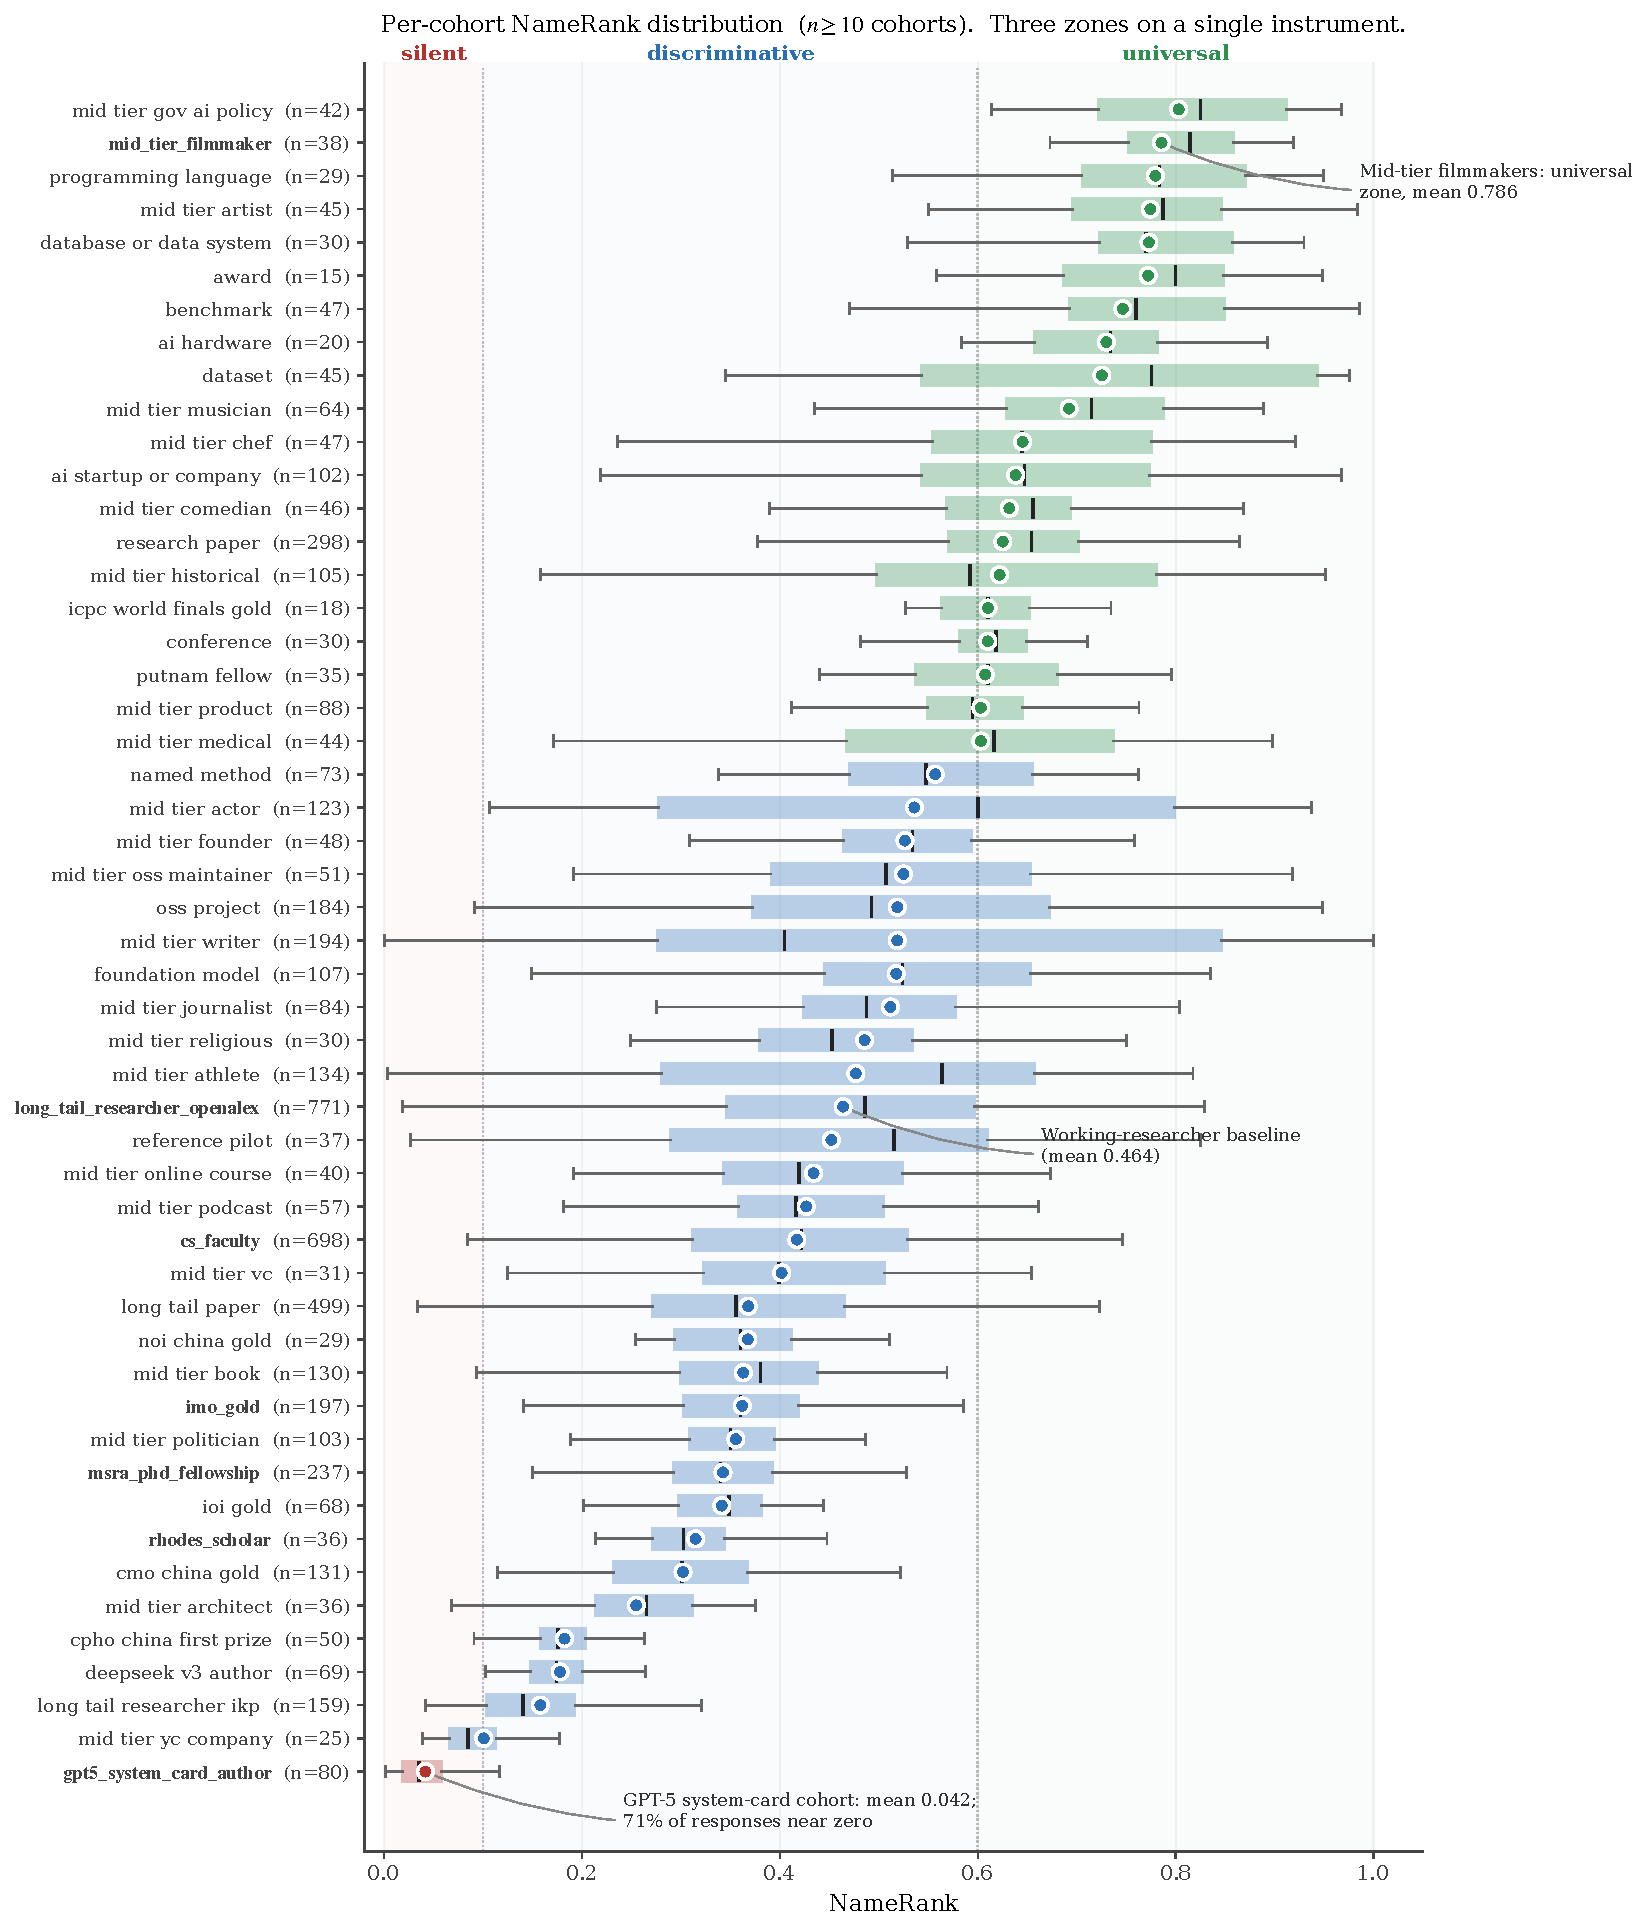
\includegraphics[width=\textwidth]{figures/fig1_cohort_distribution.pdf}
    \caption{Per-cohort NameRank distribution. Each box is a cohort ($n \geq 10$); the dot is the cohort mean, the box covers the IQR, and the inner line is the median. Three zones are visible on the same axis: \emph{silent} (mean $\leq 0.1$), \emph{discriminative} ($0.3$--$0.6$: working academics and credentialed individuals), and \emph{universal} ($> 0.7$: named artifacts and high-profile mid-tier figures). The nine credential cohorts (bold labels) cluster in the lower half of the discriminative zone (Section~\ref{sec:results-credentials}).}
    \label{fig:overview}
\end{figure}

Bibliometrics do not solve this measurement problem. In earlier work on the Incompressible Knowledge Probes (IKP) benchmark, \citet{li2026ikp} found---as a byproduct of calibrating the knowledge capacity of frontier models---that citation counts explain only about a third of the variance in whether a model recognizes a researcher. A controlled audit attributed the remainder to three corpus-level mechanisms: \emph{name uniqueness}, \emph{named-artifact attachment}, and \emph{subfield-ecosystem density}. That work characterized the residual but did not measure it: its recognition scores live on a coarse tier ladder built for parameter estimation, not for comparing entities. We take the opposite stance---the residual is the quantity of interest---and build a dedicated instrument for it. Section~\ref{sec:related} details how the instrument departs from its predecessor.

A heuristic factorization makes the target precise (a framing device, not an identity we estimate---the second factor is left unmeasured):
\begin{equation*}
\text{Recognition impact} \;\approx\; \underbrace{\text{NameRank}}_{\text{per-query presence}} \;\times\; \underbrace{\text{Query volume}}_{\text{humans querying that LLM}}
\end{equation*}
To the extent the query volume is approximately constant across entities at the relevant time horizon, the first factor carries the cross-entity variation, and it is what we measure. We do not claim NameRank measures \emph{quality} or \emph{merit}; it measures whether the corpora that mediate human curiosity at scale have internalized the entity's name.

\textbf{NameRank} is a continuous $[0,1]$ recognition score. Each entity is probed with one fixed open-ended question (``tell me what you know about [name], who [context]'') across a panel of $36$ frontier models. An independent LLM judge reads every response against a curated gold answer and returns a binary recognition verdict---true only when the response states a specific, non-guessable fact that is correct and not derivable from the context, so a fluent hallucination or a restatement of the context contributes nothing. The per-entity score is the panel recognition rate. Three properties distinguish this construction from recognition numbers that fall out of benchmark suites: it places researchers, founders, open-source maintainers, and named artifacts on a single axis; it is hallucination-resistant by construction; and cross-model disagreement is retained as a signal rather than averaged away. We evaluate $5{,}719$ entities across $54$ cohorts spanning academia, industry, open source, and the public sphere (Section~\ref{sec:method}).

\paragraph{Contributions.}
\begin{enumerate}[leftmargin=*,itemsep=1pt]
    \item A \textbf{continuous cross-domain recognition instrument} that places researchers, founders, OSS authors, public websites, and named artifacts on one $[0,1]$ axis---no prior instrument does (Section~\ref{sec:results-headline}).
    \item The \textbf{credential treadmill}: most Olympic-style intellectual credentials (IMO, IOI, CMO, Rhodes, MSRA Fellowship) score at or below a working-researcher baseline. The credential no longer propagates a name; named post-credential production does (Section~\ref{sec:results-credentials}).
    \item The \textbf{artifact-over-creator inversion}: for independent creators, the tool out-ranks its maker. The effect is measured observationally, corroborated by a context-injection experiment, and traced to an attribution-direction asymmetry in the corpus (Section~\ref{sec:results-mechanism}).
    \item \textbf{What predicts recognition}: among bibliometrics, $h$-index carries the signal---NameRank rewards name-recurrence across distinct works rather than citation volume---though even it explains under half the variance; a corpus-density gradient runs across institutions, countries, and prompt languages; and a $258$-event news cohort with a directly recorded attention ledger calibrates the instrument externally---peak salience, not persistence, drives propagation (Sections~\ref{sec:results-external}--\ref{sec:results-events}).
    \item A \textbf{validation battery} covering wording, model vintage, judge family, synthetic nulls, and gold-answer confounds (Section~\ref{sec:results-validation}); a \textbf{self-report probe} showing that pairwise recognition introspection reads the corpus prior and cannot replace verified measurement (Section~\ref{sec:results-selfreport}); and an \textbf{open release} of all probes, gold answers, responses, and code (links on page~1).
\end{enumerate}

Figure~\ref{fig:overview} previews the central result: a single recognition axis on which every cohort in the study is placed.

% ══════════════════════════════════════════════════════════════
\section{Measuring NameRank}
\label{sec:method}

Figure~\ref{fig:pipeline} summarizes the pipeline this section unpacks: a fixed open-ended probe is sent to a $36$-model panel for each entity; an independent LLM judge reads each (entity, model) response against a curated gold answer and returns a binary \emph{recognition} verdict---did the response demonstrate genuine memory of this specific entity; and the per-entity NameRank is the fraction of the panel that recognizes it.

\begin{figure}[!htbp]
    \centering
    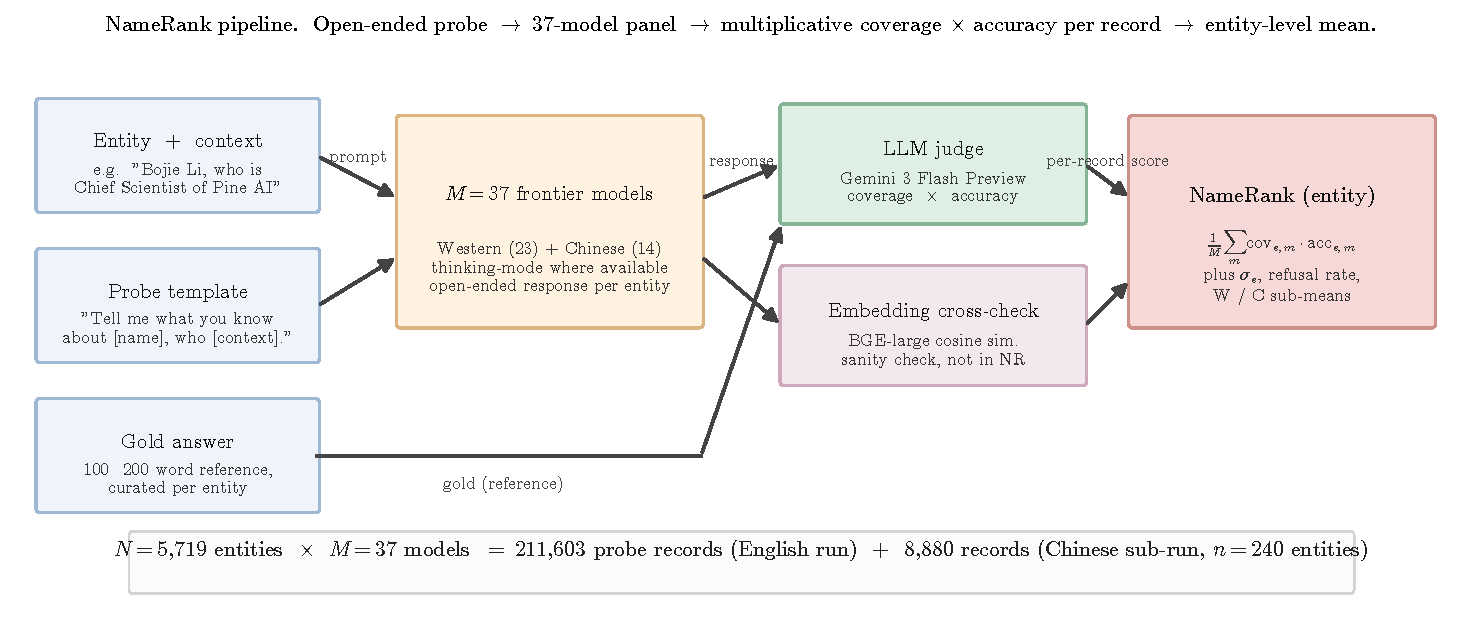
\includegraphics[width=\textwidth]{figures/fig_pipeline.pdf}
    \caption{NameRank pipeline. The probe template is fixed, with two slots: the entity name and a short role/affiliation/field context. Each of the $36$ panel models answers the open-ended probe; an LLM judge reads the response against the gold answer and returns a recognition verdict---true only if the response states at least one specific, non-guessable fact about the entity that is correct and not derivable from the context. The per-entity score is the panel recognition rate. An embedding similarity (BAAI/bge-large-en-v1.5) and a graded coverage$\times$accuracy score are stored per record as diagnostics only---neither enters the headline score (Appendix~\ref{app:scoring}). Totals: \tbd{$N$ records} over \tbd{$N$ entities}, plus a Chinese-prompt sub-run.}
    \label{fig:pipeline}
\end{figure}

\subsection{Definition}
\label{sec:construct}

For an entity $e$ with a disambiguating context $c(e)$ and a curated gold answer $g(e)$, and a model panel $\mathcal{M}$ of size $M = 36$, NameRank is the fraction of the panel that recognizes the entity,
\begin{equation}
\mathrm{NameRank}(e) \;=\; \frac{1}{M} \sum_{m \in \mathcal{M}} \mathrm{rec}(r_{e,m},\, c(e),\, g(e)),
\label{eq:namerank}
\end{equation}
where $r_{e,m}$ is the response of model $m$ to the open-ended probe
\begin{quote}
\small ``\emph{Tell me what you know about [name], who [context]. If you do not recognize this entity, respond with `unknown'. Limit your response to about 150 words.}''
\end{quote}
and $\mathrm{rec} \in \{0,1\}$ is a recognition verdict produced by an LLM judge (Section~\ref{sec:method-judge}): it is $1$ only when the response states at least one \emph{specific, non-guessable} fact that is true of this exact entity---verified against the gold answer or the judge's own knowledge---and not derivable from the disambiguating context. A refusal, a hedged non-answer, a response confined to context-derivable generalities, and a fluent but wrong-person biography all score $0$. NameRank thus reads as the probability that a randomly drawn frontier model genuinely knows the entity. Three worked (entity, model, response) triples spanning the range are provided in the \repodoc{worked-examples.md}{repository documentation}.

\subsection{Probe Design}
\label{sec:probe}

\textbf{One open-ended probe per entity.} Closed-factoid probes have a known failure mode: a model that recognizes the entity through fact $X$ but does not recall fact $Y$ scores zero on a probe-of-$Y$, biasing the metric toward specific-fact recall. The open-ended probe instead asks the holistic question: does the model have a retrievable representation of this entity? The template is fixed, with two slots: the canonical entity name, and a short disambiguating clause giving role, affiliation, and field (e.g., \emph{``Wei Zhang, who is a professor of mathematics at MIT working on PDEs''}). The context resolves name collisions at probe time without revealing the gold answer. The full English and Chinese probe text and the judge prompt are reproduced verbatim in the \repodoc{probe-templates.md}{repository documentation}.

The context names role, affiliation, and field---never specific contributions, papers, dates, or named artifacts---so it anchors disambiguation without leaking the gold; the judge's rubric credits only specific named facts, and generic in-context biographies earn nothing (evidence in Appendix~\ref{app:spec}; a dedicated context-ablation in Appendix~\ref{app:confounds}).

\subsection{Gold Answers}
\label{sec:gold}

For each entity we construct a gold answer built from \emph{entity-specific, verifiable facts}---named works, named contributions, real affiliations with dates, and other identifying particulars---composed from primary and authoritative sources: bibliographic records (OpenAlex, Semantic Scholar, Crossref) for researchers and papers, official competition and award records for credential holders, code-host metadata and READMEs for open-source artifacts, encyclopedia lead sections for public figures and companies, and length-normalized web-grounded profiles for the long tail. The gold serves two roles for the judge: it \emph{identifies} which specific entity the probe refers to (disambiguating same-name individuals), and it supplies a correctness anchor. It deliberately does \emph{not} restate the disambiguating context: a fact the probe already supplies earns no recognition credit, so the gold's discriminating content is the material a model must know independently. We audit a stratified sample against primary sources following the protocol of \citet{li2026ikp}; the observed correction rate is small, typically year-of-affiliation drift. A confound check confirms NameRank does not reduce to a has-a-Wikipedia-page flag (Appendix~\ref{app:confounds}).

\subsection{The Judge}
\label{sec:method-judge}

We use Gemini~3 Flash Preview as the judge (direct Google API to minimize routing variance; temperature $0$). The judge is shown the entity name, the probe context, the gold answer, and the model's response, and returns a binary \emph{recognized} verdict. It is instructed to credit recognition only when the response states a specific, non-guessable fact that is (a)~true of this exact entity, established either by the gold answer or by the judge's own reliable knowledge; (b)~not derivable from the probe context; and (c)~about the same entity the gold identifies, not a same-name individual. The judge uses knowledge \emph{asymmetrically}: it may refute freely---flagging a wrong-person biography or a false claim using anything it knows---but it may \emph{credit} a fact only when it positively verifies it, so a plausible-sounding but unverified specific about an entity it does not recognize counts for nothing (the signature of hallucination on obscure or fictional names). For competition participants, fellowship recipients, and minor-paper authors---where an LLM judge has no reliable per-individual memory---an anti-confabulation provision restricts credit to facts present in the gold or to major, widely-documented achievements, never to fine-grained particulars asserted from the judge's own memory. Broad field, nationality, an employer inferable from the name, generic praise, and restatements of the context are all non-credit by construction.

We also record, per response, a graded coverage$\times$accuracy score and the embedding cosine similarity to the gold~\citep{bge2024}; both are retained as diagnostics and neither enters the headline NameRank. Appendix~\ref{app:scoring} shows why a judge is required---embedding similarity credits fluent hallucinations as recognized---and why the recognition verdict is preferred to a graded score: graded coverage measures overlap between two arbitrary samples of an entity's fact universe, penalizing a model that knows the entity through facts the gold happens to omit, whereas recognition asks the construct-faithful question of whether the model knows the entity at all. The dependence of the findings on the judge's model family is quantified with a multi-judge re-grade in Appendix~\ref{app:cross-judge}.

\subsection{Aggregation}
\label{sec:aggregation}

NameRank is the unweighted panel recognition rate across the $36$-model panel (Equation~\ref{eq:namerank}). We also retain, per entity, the refusal rate, the Western/Chinese sub-panel rates, the diagnostic graded score, and the raw response text. Averaging across the panel is what makes the score stable: a single model contributes noise from prompt sensitivity, refusal-policy idiosyncrasies, and training-data accidents, while the panel rate integrates corpus presence over the current frontier fleet. The retained per-model verdicts keep the residual signal---an entity recognized by one vendor's models but not another's is itself informative (Section~\ref{sec:results-language}). A synthetic-null floor---fictional entities built on each cohort's gold recipe and scored by the same judge---calibrates the residual recognition a name that exists in no corpus can attract; scores are read against this floor (Appendix~\ref{app:synthetic}).

\subsection{Model Panel}
\label{sec:panel}

The panel comprises $36$ frontier and near-frontier models accessed via OpenRouter and direct vendor APIs, spanning Western and Chinese vendors and frontier-reasoning to small (sub-$30$B) classes (full roster in Appendix~\ref{app:spec}, Table~\ref{tab:panel}). Thinking mode is enabled wherever a thinking variant exists: for a recognition metric, thinking mode is the operational mode in which most user queries are answered, so the panel reflects deployment reality. The Western/Chinese partition is used only for the cross-vendor analysis (Section~\ref{sec:results-language}); the headline NameRank is the unweighted mean over all $36$ models.

\subsection{Entity Cohorts}
\label{sec:cohorts}

We evaluate \tbd{$N$} entities in \tbd{$K$} cohorts spanning credentialed individuals (olympiad medalists, Putnam, ICPC, Rhodes, MSRA fellows), working academics, industry figures, named artifacts, mid-tier cross-profession figures (writers, athletes, actors, chefs, podcasts), a hand-curated diagnostic reference set (public figures, engineers, and artifacts used for case-level analyses), and special cohorts (technical-report and system-card author lists, conferences, awards, and LLM-area figures---method originators, foundational-paper authors, and best-paper-award recipients). The design goal is coverage of the axes the metric claims to unify: credentialed individuals whose recognition should be carried by the credential if credentials propagate; working academics with known bibliometrics, as the external-validity anchor; industry figures whom no bibliometric measures; named artifacts, to compare things against their makers; and mid-tier figures, to test the axis outside the technology world. The per-group breakdown is in Appendix~\ref{app:spec} (Table~\ref{tab:cohort-groups}); full per-cohort sizes, rates, and inclusion criteria are in the \repodoc{cohorts.md}{released cohort specification}.

\subsection{Cross-Language Sub-Run, Execution, and Release}
\label{sec:execution}

A subset of entities---the diagnostic reference set, the Chinese olympiad and fellowship cohorts, the technical-report author cohort, and small Western control samples---was re-probed with the Chinese-translated template (gold answers and judge prompt remain English, since the judge grades across languages; cohort selection detail in Appendix~\ref{app:cross-lang}). A parallel Python runner drives the probe and judge stages. We release the probe specifications, all gold answers, all judged response records, the Chinese sub-run, and the analysis pipeline at \url{https://github.com/19PINE-AI/namerank} (companion website: \url{https://01.me/research/namerank}).

\subsection{Scope: What NameRank Does and Does Not Measure}
\label{sec:scope}

NameRank is not a quality, merit, or intrinsic-impact metric. It measures \emph{the propagation of a specific name into the indexed corpora that frontier-model training pipelines scrape}. This correlates with academic impact through bibliometric mechanisms, with cultural reach through named-artifact attachment, and with both through derivative-content density (tutorials, blog posts, talks, podcast mentions)---but it does not measure the underlying work. The clearest counterexample in our data is a Chinese-language visa-monitoring website with roughly a million users whose NameRank is nonetheless low, because its name never co-travels with its creator's in indexable text (Section~\ref{sec:results-cases}). The metric correctly registers low there, not because the artifact lacks impact, but because the metric measures something specific. We treat this as a feature: a clean instrument reports what it measures, not what users wish it measured.

Three empirical properties, each established later, govern how the score should be read. First, the axis is meaningful \emph{across} domains: researchers, founders, OSS authors, and artifacts land on one scale (Section~\ref{sec:results-headline}). Second, below the corpus-presence threshold the metric is largely \emph{silent rather than misleading}---the panel refuses or withholds recognition instead of producing spurious rankings---against a synthetic-null floor calibrated per gold recipe (Section~\ref{sec:results-headline}, Appendix~\ref{app:synthetic}). Third, the score directly captures the residual that bibliometrics leave unexplained: for a working researcher, one widely-used, cleanly-named open-source tool moves NameRank more than one well-cited paper (Sections~\ref{sec:results-mechanism}, \ref{sec:results-external}).

% ══════════════════════════════════════════════════════════════
\section{Results}
\label{sec:results}

\tbd{This section is being regenerated on the final run. The subsections and
their labels below are fixed; each will be filled with the recognition-rate
results, tables, and figures. A one-line statement of the finding each will
report is given as a placeholder.}

\subsection{A Single Axis Across Domains}
\label{sec:results-headline}
\tbd{Researchers, founders, OSS authors, and named artifacts placed on one
recognition axis; the three zones (silent / discriminative / universal) and the
cross-domain placement table.}

\subsection{The Credential Treadmill}
\label{sec:results-credentials}
\tbd{Olympic-style credentials (IMO, IOI, NOI, CMO, Rhodes, MSRA) at or below
the working-researcher baseline; the credential no longer propagates a name,
named post-credential production does. Ladder in Figure~\ref{fig:credentials}.}

\subsection{The Treadmill Inverts at the Marquee Tier}
\label{sec:results-awards}
\tbd{Marquee late-career prizes (Nobel, Turing, Fields) clear the baseline and
accrue for decades, unlike early credentials. Ladder in Figure~\ref{fig:awards};
detail in Appendix~\ref{app:awards}.}

\subsection{Named-Artifact Amplification}
\label{sec:results-mechanism}
\tbd{For independent creators of single artifacts, the tool out-ranks its maker.
Inversion and injection in Figure~\ref{fig:inversion}.}

\subsubsection{The artifact-over-creator inversion}
\tbd{Verified (creator, artifact) pairs; the artifact out-ranks the creator in
most independent-creator pairs.}

\subsubsection{Attribution flows from creator to artifact, not back}
\label{sec:asymmetry-body}
\tbd{Directional mention-rate asymmetry (creator to artifact vs.\ artifact to
creator) across the pair regimes.}

\subsubsection{A worked case: Tianshou and its author}
\label{sec:results-tianshou}
\tbd{Jiayi Weng vs.\ OpenAI IC peers; artifact-mediated recognition; survives
translation.}

\subsubsection{Context injection corroborates the mechanism}
\label{sec:results-mediation-causal}
\tbd{Naming the artifact in the creator's context lifts recognition where the
panel barely stores the creator; capability gradient.}

\subsection{What Predicts NameRank}
\label{sec:results-external}
\tbd{Bibliometric, institutional, and geographic correlates of recognition.}

\subsubsection{Among bibliometrics, $h$-index carries the signal---and still explains under half the variance}
\tbd{$h$-index dominates raw citations; citations add no marginal signal;
most variance remains unexplained. Regressions figure to be restored.}

\subsubsection{Institution and country: the corpus-density gradient}
\label{sec:results-geography}
\tbd{Top-school CS faculty recognized well above lower-corpus-density peers,
even at matched citations; country gradient in Figure~\ref{fig:country}.}

\subsubsection{Prompt language routes retrieval}
\label{sec:results-language}
\tbd{Prompt language routes retrieval into language-specific corpus pockets;
Chinese prompts lift Chinese-named cohorts.}

\subsection{News Events: The Attention Ledger}
\label{sec:results-events}
\tbd{On $258$ news events with pageview ledgers, recognition tracks attention
dose and loads on peak salience rather than persistence; templated series names
dilute. Figure and full regressions.}

\subsection{Boundary Condition: Reach Without Name Propagation}
\label{sec:results-cases}
\tbd{tuixue.online---largest human reach, lowest recognition---dissociates reach
from name propagation; symmetric across languages.}

\subsection{Self-Reported Recognition: Asking a Model Is Not Measuring It}
\label{sec:results-selfreport}
\tbd{Models asked to rank their own recognition recover the panel ordering only
partially ($\rho \approx 0.5$--$0.6$); self-report reads a shared corpus prior,
not the model's own state, but rarely claims a fictional name.}

% Placeholder floats: labels referenced from the appendix are defined here so
% cross-references resolve until the figures are regenerated on the final run.
\begin{figure}[!htbp]\centering\fbox{\tbd{credential ladder figure}}
\caption{\tbd{The credential treadmill: cohort recognition rates against the
working-researcher baseline.}}\label{fig:credentials}\end{figure}

\begin{figure}[!htbp]\centering\fbox{\tbd{award ladder figure}}
\caption{\tbd{Marquee prizes clear the baseline and accrue over decades.}}
\label{fig:awards}\end{figure}

\begin{figure}[!htbp]\centering\fbox{\tbd{artifact--creator inversion figure}}
\caption{\tbd{Named-artifact amplification: creator vs.\ artifact recognition
and the context-injection lift.}}\label{fig:inversion}\end{figure}

\begin{figure}[!htbp]\centering\fbox{\tbd{country gradient figure}}
\caption{\tbd{Country gradient in CS-faculty recognition.}}
\label{fig:country}\end{figure}


% ══════════════════════════════════════════════════════════════
\section{Robustness and Validation}
\label{sec:results-validation}

The findings above rest on three design choices---an LLM judge over embedding similarity, a binary recognition verdict over a graded score, and open-ended over closed-factoid probes---and on the headline numbers not being artifacts of wording, model vintage, judge family, or gold-answer construction. Table~\ref{tab:threats} summarizes the validation battery; Appendices~\ref{app:scoring}--\ref{app:confounds} give the full evidence. Three results carry most of the weight.

\begin{table}[!htbp]
\centering
\small
\caption{The validation battery: each threat to the findings, the check run against it, and the outcome. Full tables and figures in the referenced appendices.}
\label{tab:threats}
\begin{tabular}{>{\raggedright\arraybackslash}p{3.5cm}>{\raggedright\arraybackslash}p{3.8cm}>{\raggedright\arraybackslash}p{5.5cm}c}
\toprule
\textbf{Threat} & \textbf{Check} & \textbf{Outcome} & \\
\midrule
Score reflects panel composition, not the entity & Variance decomposition over all $211{,}603$ records; disjoint-panel re-score of the event cohort & Entity variance ${\approx}3.3\times$ model variance; eight $2026$ replacement models rank events at $r = 0.905$ with the surviving panel (\S\ref{sec:results-events}) & App.~\ref{app:scoring} \\
Fluent hallucinators inflate scores & Refusal and generosity structure across the panel & Accuracy axis zeroes wrong-person bios; refusal rate tracks the silent zone & App.~\ref{app:scoring} \\
A judge-free embedding score would suffice & Judge-vs-embedding comparison, $175$K records & Embedding similarity is flat across judge scores and credits hallucinations & App.~\ref{app:scoring} \\
Findings are an artifact of probe wording & Four-template re-probe, $29{,}600$ records & Rankings invariant ($r \geq 0.93$); absolute levels are template-conditional & App.~\ref{app:prompt-sensitivity} \\
The silent zone is corpus timing, not obscurity & Training-cutoff natural experiment & Matched difference-in-differences ${\approx}0$; silence is intrinsic & App.~\ref{app:cutoff} \\
Findings depend on the judge's model family & Three-judge re-grade, $615$ records & Judges agree ($r = 0.87$--$0.93$); small own-family lift moves no finding & App.~\ref{app:cross-judge} \\
Unknown names could score above zero & $30$ fictional entities through the full pipeline & Floor ${\approx}0.04$ (dense golds), ${\approx}0.20$ (boilerplate golds); adjusting for it \emph{widens} the credential gap & App.~\ref{app:synthetic} \\
Gold length, context leakage, Wikipedia presence, or web attention drive the results & Dedicated ablations and regressions; $24$-month pageview baseline & All four rejected & App.~\ref{app:confounds} \\
\bottomrule
\end{tabular}
\end{table}

\textbf{The scoring rule is load-bearing.} Across all records, the entity factor explains far more of the variance than the model factor does, and an entirely disjoint replacement panel reproduces the event ordering---the score measures the entity, not the fleet. The refusal structure shows why a recognition verdict is required: the zero-refusal models are fluent hallucinators that always produce a confident wrong-person biography, which the verdict scores as non-recognition, while embedding similarity---flat across judge-score buckets---would credit exactly those bios as recognized (Appendix~\ref{app:scoring}).

\textbf{Orderings survive wording, vintage, and judge; levels do not.} Re-probing under three paraphrased templates leaves the entity ordering and every cohort-level finding intact while shifting absolute levels, so NameRank values are template-conditional (Appendix~\ref{app:prompt-sensitivity}). A training-cutoff natural experiment on two contemporaneously-published author cohorts shows the silent zone is intrinsic rather than corpus timing---but also reveals a ${\sim}0.13$/yr cross-vintage drift, so longitudinal claims must be made on within-run \emph{relative} gaps (Appendix~\ref{app:cutoff}); the thresholded behavior itself is what the transformer fact-storage literature predicts~\citep{geva2021transformer, petroni2019language, kandpal2023, overshadow2025}. And a three-judge re-grade (Gemini, Claude, GPT-5) preserves every finding, with only a small own-family scoring lift that shifts per-vendor tables (Appendix~\ref{app:cross-judge}).

\textbf{Floors are calibrated and confounds rejected.} Thirty fictional entities establish the noise floor: near-zero for dense golds, elevated for boilerplate golds---and floor-adjusting \emph{widens} the credential gap (Appendix~\ref{app:synthetic}). Dedicated ablations reject gold-answer length, context leakage, and Wikipedia presence or attention as alternative explanations: NameRank is not a has-a-Wikipedia-page flag---the binary flag explains ${\sim}2\%$ of long-tail variance against ${\sim}40\%$ for $h$-index---and it is not pageview rank, which is undefined for $71\%$ of entities and explains $R^2 = 0.06$ where defined (Appendix~\ref{app:confounds}).

% ══════════════════════════════════════════════════════════════
\section{Discussion}
\label{sec:discussion}

\subsection{What We Have Built and What We Have Not}

NameRank is a continuous cross-domain instrument with empirical threshold cleanliness, validated external correlates ($h$-index, institution, the event attention ledger), and mechanism-level structure. It is suitable for cross-domain placement on a common scale, for tracking name propagation into training corpora over time, and for measuring the recognition channel that bibliometrics miss. It is not a quality metric (it measures what models absorbed, not what is worth absorbing), not an attribution system (the name, not the deed), and not predictive of anything the corpus has not yet recorded.

\subsection{The Credential Treadmill Thesis in Context}
\label{sec:discussion-credentials}

The credential treadmill does not contradict the olympiad-outcome literature, which finds medals causally raise subsequent \emph{academic productivity}~\citep{agarwalGaule2020, smpy2020}; our dependent variable is different. When it is name-propagation into LLM corpora rather than paper count, the credential per se is a near-zero predictor---continued production of named, indexable artifacts is what propagates. The credential still signals ability and motivation; only its role as a name-propagation channel has shrunk. In the language of signaling theory~\citep{spence1973}, the LLM-corpus channel transmits not the credential itself but the named, indexable production that may follow it.

\subsection{What Clock Does NameRank Read? Lifetime vs.\ Current-Term Recognition}
\label{sec:discussion-clock}

A recognition score could measure two different quantities: \emph{cumulative} presence---everything a name has deposited in the corpus over a career---or \emph{current-term} salience, what the world is paying attention to now. Three findings established independently above jointly place NameRank in the first category. Within IMO gold medalists, medal year is uncorrelated with the score (Pearson $-0.04$ over $2005$--$2015$; Appendix~\ref{app:credentials}): recognition neither fades for older medalists nor spikes for recent ones. MSRA fellowship cohorts show the complementary shape---five-year-cohort means rise from $0.312$ ($2005$--$2009$) to $0.382$ ($2015$--$2019$) and dip only for the $2020$--$2024$ fellows---exactly what an integral over post-credential production looks like when the newest cohorts have not yet had time to produce (Appendix~\ref{app:credentials}). And on news events, where attention is directly recorded, the score loads on \emph{peak} salience rather than persistence (Section~\ref{sec:results-events}): what matters is how many name-bearing documents were minted, not how long the audience stayed. Read together: NameRank is a cumulative ledger of name-bearing text, snapshotted through the current model fleet---a lifetime measure weighted by documentation density, not a barometer of current attention. Current-term change is accessible only longitudinally, as within-run relative gaps across successive fleets (Section~\ref{sec:predictions}).

\subsection{\texorpdfstring{The Artifact $>$ Creator Inversion and the Anonymity-of-Tooling Problem}{The Artifact > Creator Inversion and the Anonymity-of-Tooling Problem}}

For independent creators of well-named single artifacts the tool out-ranks its maker (Section~\ref{sec:results-mechanism}), and the context-injection experiment is consistent with this being a causal effect (modulo a coverage-echo confound we bound but do not fully remove, Section~\ref{sec:results-mediation-causal}). The mechanism is attribution-direction asymmetry: creator-bios feature their creations, but artifact-discussion text (OSS docs, tutorials, papers) names the artifact far more often than the creator. The actionable consequence is uncomfortable but concrete: for propagating a name through the LLM channel, building a clearly-named tool beats writing many papers---yet the lift accrues to the tool's name first and to the creator only through it, so a tool buried under generic corporate branding yields no personal NameRank.

\subsection{What Raises Recognition---and Whether Going Viral Helps}
\label{sec:discussion-implications}

Read prescriptively, the findings converge on a single lever: recognition accrues to \emph{distinctively-named, indexable production accumulated over a career}. Volume of name-bearing works dominates citation weight ($h$-index over raw citations, Section~\ref{sec:results-external}); one clearly-named artifact outperforms many papers (Section~\ref{sec:results-mechanism}); and only the marquee credential tier propagates on its own, mid-career honors do not (Section~\ref{sec:results-awards}). Because the ledger is cumulative (Section~\ref{sec:discussion-clock}), the effective strategy is long-horizon and structural rather than about any single achievement: keep depositing documents that carry a distinctive, low-collision name into English-indexed text.

This also bounds what public attention buys. Going viral helps only insofar as the spike is \emph{captured as durable, name-bearing documents}: on news events the score loads on peak salience over persistence and enters through the accuracy channel, not raw coverage (Section~\ref{sec:results-events}), so a burst that mints many correct name-attached records converts while ephemeral engagement that leaves none does not---and even captured attention decays (the $-0.049$ vintage echo). The conversion is category-dependent: within celebrity cohorts pageviews track NameRank strongly, but for technical creators attention \emph{flow} and corpus \emph{stock} decouple and can invert (Appendix~\ref{app:confounds}; a $6.4$K-pageview library outscores a million-pageview model). Attention is thus a means, valuable only when it deposits distinctively-named text into the corpus---never an end in itself.

\subsection{The Corpus-Density Gradient and Its Limits}

Section~\ref{sec:results-geography} documents a twofold Stanford--Tsinghua recognition gap that recurs at country scale, with the well-sampled USA-over-China-over-India ordering as its firm backbone and the small-country leaders as suggestive only. The mechanism is English-corpus density; the consequence is structural inequality in name propagation per unit of research output.

Three caveats: the bottom-of-ladder institution samples are small ($n = 4$); uncorrected researcher mobility inflates the US average and depresses China's; and the gradient is downstream of the indexing and crawling decisions of training-data pipelines, so it could in principle be reduced by changing them. Within the current corpus regime, it is a substantial structural effect.

\subsection{Inherited Demographic Biases}
\label{sec:discussion-bias}

NameRank inherits the demographic biases of its judge and probed models, and measures them faithfully rather than correcting them. \citet{li2026ikp} documented a ${\sim}2\times$ recognition attenuation for common East-Asian surnames; we find a second, smaller effect on first-name-inferred gender: within the researcher cohorts---where institution matching and $h$-index-decile adjustment are available and survive---man-coded names outscore woman-coded names by roughly $0.03$--$0.05$ (Appendix~\ref{app:gender}). We restrict the claim to that controlled comparison: the much larger raw gaps in cross-profession cohorts reflect real fame differences among the sampled individuals, not a NameRank artifact. As with the surname effect, the gender gap is an inherited property of the corpus-and-judge stack that NameRank reports, not a calibration target; downstream uses must account for it.

\subsection{Limitations}

Appendix~\ref{app:limitations} tabulates every caveat with its direction and mitigation. The material ones: absolute levels are wording- and gold-conditional while rankings are robust; the full run uses a single judge with a small own-family lift; only within-run \emph{relative} gaps are comparable across model fleets (${\sim}0.13$/yr vintage drift); and the context-injection lift is an upper bound on named-artifact amplification.

\subsection{Registered Predictions for Future Re-Runs}
\label{sec:predictions}

NameRank is a snapshot, so a re-run each release cycle yields a longitudinal trajectory. Because of the ${\sim}0.13$/yr vintage drift, we state predictions as within-run \emph{relative} gaps (so the drift cancels) and register four falsifiable ones for the 2027 fleet: (i)~the IMO-gold-vs-OpenAlex gap widens from $-0.102$ to $\leq -0.13$ within 12 months (named-artifact-attached careers accumulate text, credential-only cohorts do not); (ii)~the median artifact-minus-creator delta on independent-creator pairs grows from $+0.09$ to $\geq +0.14$ within 18 months; (iii)~the Stanford-vs-Tsinghua gap narrows by $\geq 25\%$ but does not close within 24 months as Chinese-language training data enters frontier models; (iv)~on a re-run of the news-event cohort (Section~\ref{sec:results-events})---the cleanest of the four, since its exposure side is frozen in the pageview archive---the $2023$-vs-$2021$ vintage gap ($-0.049$ at matched attention) shrinks by at least half within 18 months as post-event derivative text accumulates.

% ══════════════════════════════════════════════════════════════
\section{Related Work}
\label{sec:related}

\subsection{Relation to the Predecessor Instrument}

The direct predecessor of this work is the recognition analysis in the IKP benchmark \citep[\S5.7]{li2026ikp}, which established the findings this paper builds on: on $345$ CS-researcher probes, $\log(\text{citations})$ explains only ${\sim}35\%$ of recognition variance, with the remainder attributed in a controlled audit to \emph{named-artifact amplification}, \emph{name uniqueness} (common East Asian surnames attenuate recognition by ${\sim}2\times$), and \emph{subfield-ecosystem density}; and on $557$ Wikidata-grounded probes, domain-specific recognition multipliers trace to the structure of web discourse around each fact type rather than to entity prominence. IKP nonetheless treated recognition as a benchmark byproduct. NameRank differs in each dimension that matters for an impact metric: a $[0,1]$ recognition rate over a $36$-model panel (vs.\ a six-landmark tier ladder calibrated for parameter estimation); thousands of entities across dozens of cohorts spanning industry, OSS, and mid-tier figures (vs.\ $345$ researchers and $557$ Wikidata probes); open-ended probes scored by a per-model recognition verdict (vs.\ closed-factoid binary verdicts); $h$-index rather than raw citations as the validated bibliometric correlate; and cross-model variance retained as signal rather than absorbed into a tier label.

\subsection{Scientometric Measures of Researcher Impact}

The classical instruments for researcher impact---citation count, $h$-index~\citep{hirsch2005index}, journal impact factor---measure intellectual reach within the academic publication system, and are increasingly understood as failing under pressures relevant here: authorship-list inflation and uneven attribution~\citep{lariviere2019}, the \emph{hyperauthorship} problem of pricing contributions to thousand-author papers~\citep{cronin2001hyperauthorship} (a GPT-4 co-author's citation count is mechanically large but says nothing about name-recognition), prestige-hierarchy biases spanning an order of magnitude across institutional tiers~\citep{wapman2022quantifying}, and within-researcher variance that motivates decompositions like the $Q$ parameter~\citep{sinatra2016quantifying}.

None of these instruments cross the academic boundary cleanly. Citation count does not measure Sam Altman, Aravind Srinivas, or a Walmart CTO; $h$-index does not measure the creator of nanoGPT. Bespoke domain metrics (Google PageRank for websites, GitHub stars for OSS, Spotify monthly listeners for musicians, IMDb scores for film) do not interconvert. Collective-attention metrics do---search volume, Google Trends, and Wikipedia pageviews place any entity on one axis, and pageviews in particular are an established salience proxy~\citep{mestyan2013early,ripberger2011capturing}---but they count queries and article traffic rather than verified knowledge, and they are empirically near-orthogonal to NameRank: undefined off Wikipedia, weakly predictive where defined, and negatively correlated within technical cohorts (Appendix~\ref{app:confounds}). We use attention records as calibration input on the event cohort (Section~\ref{sec:results-events}), not as the measurand: NameRank reads the \emph{outcome} of the training pipeline---what deployed models can correctly state---rather than the exposure that feeds it. The cross-domain measurement of eminence has a long prior tradition in \emph{historiometry}~\citep{simonton1999}, which quantifies the reputational standing of eminent individuals from archival traces; NameRank can be read as a historiometric instrument whose archive is the frontier-model training corpus rather than biographical dictionaries and citation indices. For impact assessment that spans academia, industry, OSS, and the long tail of solo operators, a cross-domain instrument is needed; NameRank is the first we are aware of that reads this archive directly.

\subsection{LLM-as-Judge for Quality and Impact}

\citet{thelwall2024chatgpt, thelwall2025plos, thelwall2025multistage} use ChatGPT to score paper \emph{quality} against the UK REF rubric; \citet{kousha2025jasist} extend to societal influence; \citet{liu2026llmprediction} forecast citation counts. These differ from NameRank in two respects: they ask the LLM to \emph{judge} quality, where we ask what the model has \emph{absorbed}; and they average within a single model across iterations, where we average across the full $36$-model panel, treating cross-model variance as signal.

A separate line asks whether models \emph{know what they know}: self-assessed confidence is well calibrated on aggregate question answering \citep{kadavath2022language} but degrades at the boundary of a model's own competence \citep{yin2023selfaware}, and entity popularity modulates factual reliability \citep{mallen2023trust}. Section~\ref{sec:results-selfreport} adds an entity-level counterpart: pairwise self-reported recognition, aggregated with the Bradley--Terry machinery familiar from Chatbot Arena \citep{chiang2024chatbot}, tracks the corpus salience shared across vendors rather than the reporting model's own verified knowledge.

The known LLM bias most relevant to our setting is the \emph{Matthew effect}~\citep{merton1968matthew} as it propagates through LLM training corpora: frontier models recall already-highly-cited work disproportionately, inflating the rich-get-richer dynamic familiar from the bibliometrics literature. We inherit this bias and treat it as a known property of the measurand---NameRank measures \emph{what frontier models have absorbed}, which is itself shaped by the Matthew dynamic. The bias is part of what we measure, not a flaw to be corrected.

\subsection{Credentials and Long-Run Outcomes}

A longitudinal literature finds that early mathematical talent and olympiad medals predict---and causally raise---later \emph{academic} productivity: the 50-year SMPY study~\citep{smpy2020}, a medal-cutoff natural experiment~\citep{agarwalGaule2020}, and work documenting substantial within-elite heterogeneity~\citep{guellich2025}. Our credential-treadmill finding does not contradict this literature; it changes the dependent variable from academic production to LLM-mediated name recognition and finds that the credential per se carries little of it (Sections~\ref{sec:results-credentials}, \ref{sec:discussion-credentials}).

% ══════════════════════════════════════════════════════════════
\section{Conclusion}
\label{sec:conclusion}

NameRank operationalizes the $65\%$ recognition-variance residual that \citet{li2026ikp} characterized but did not measure: a cross-domain, hallucination-resistant recognition rate over a $36$-model panel. Its findings each subvert a default expectation---olympiad credentials no longer propagate names, named tools out-rank their makers, the structure of citation production beats its volume, on news events, where world attention is directly recorded, peak salience rather than persistence drives propagation, and asking a model to rank its own recognition returns the shared corpus prior rather than its own knowledge state---and each is mechanistically grounded and survives a battery of robustness checks. The broader claim is that human curiosity about people and artifacts is now re-mediated by a few frontier models, and whether a name has propagated into their training corpora is itself a measurable quantity. Three uses follow: a cross-domain impact metric (a Walmart CTO at $0.52$ is directly comparable to a Stanford professor at $0.54$), a longitudinal tracker of how discourse reaches training pipelines, and a normative indicator for career strategy (build and name your own tool). All probes, gold answers, responses, and code are released at \url{https://github.com/19PINE-AI/namerank}; companion site \url{https://01.me/research/namerank}.

% ══════════════════════════════════════════════════════════════
\section*{Acknowledgements}

This paper was produced using Pine Copilot's voice-directed \emph{whisper coding} workflow~\citep{pineai2026whispercoding}, in which the authors specify, discuss, and review the work by voice while a coding agent---Claude Code with Claude Opus 4.8 and Claude Fable 5---carries out the planning, coding, experiments, and paper writing.
We thank BSQL Networking for hosting the NVIDIA RTX PRO 6000 GPU.

% ══════════════════════════════════════════════════════════════
\bibliographystyle{plainnat}
\bibliography{references}

\clearpage
\appendix
% ══════════════════════════════════════════════════════════════
\section{Credential Ladder Detail}
\label{app:credentials}

Table~\ref{tab:credential-treadmill} gives the full credential ladder summarized in Figure~\ref{fig:credentials}.

\begin{table}[!htbp]
\centering
\small
\caption{Credential ladder. The OpenAlex long-tail researcher cohort ($n = 771$, citations $500$--$30{,}000$) supplies the working-researcher baseline. The two rows marked $\dagger$ are large-team co-authorship cohorts shown for context, not credentials, and are excluded from the ``$7$ of $9$'' count.}
\label{tab:credential-treadmill}
\begin{tabular}{lrrr}
\toprule
Credential & $n$ & Mean NameRank & vs.\ baseline \\
\midrule
ICPC World Finalist gold & 18 & 0.610 & $+0.146$ \\
Putnam top-25 fellow & 35 & 0.608 & $+0.144$ \\
\textbf{OpenAlex long-tail researchers (baseline)} & \textbf{771} & \textbf{0.464} & --- \\
NOI China gold & 29 & 0.368 & $-0.096$ \\
\textbf{IMO gold (2005--2015)} & \textbf{197} & \textbf{0.362} & $\mathbf{-0.102}$ \\
MSRA PhD Fellowship & 237 & 0.343 & $-0.121$ \\
IOI gold & 68 & 0.341 & $-0.123$ \\
Rhodes Scholarship & 36 & 0.315 & $-0.149$ \\
CMO China gold & 131 & 0.302 & $-0.162$ \\
CPhO China first prize & 50 & 0.182 & $-0.282$ \\
DeepSeek-V3 paper author$^\dagger$ & 69 & 0.178 & $-0.286$ \\
GPT-5 system-card author$^\dagger$ & 80 & 0.042 & $-0.422$ \\
\bottomrule
\end{tabular}
\end{table}

\textbf{Career-track split.} Within IMO gold medalists, US-tracked academic/industry careers---the subset most comparable to the citation-floored OpenAlex baseline---score ${\sim}0.50$; non-Anglophone-tracked golds score ${\sim}0.30$. The medal-and-name pair propagates only where the post-medal career produces English text.

\textbf{Temporal patterns.} Within MSRA fellows, five-year-cohort means rise from $0.312$ (2005--2009) to $0.337$ (2010--2014) to $0.382$ (2015--2019) and dip to $0.343$ (2020--2024), consistent with recent fellows having had less time for post-fellowship production to propagate. Within IMO 2005--2015, Pearson(year, NameRank) $= -0.042$, indistinguishable from zero: the credential signal neither strengthens nor decays within the ten-year window.

% ══════════════════════════════════════════════════════════════
\section{Conditional-Probe Asymmetry Details}
\label{app:asymmetry}

For each of the $11$ verified (creator, artifact) pairs, the full per-model breakdown of $C\!\to\!A$ and $A\!\to\!C$ (fraction of non-refusal model responses that name the counterpart) is released as a supplementary CSV.

\textbf{Per-model mention table for Jiayi Weng / Tianshou.} Of the $28$ non-refusal responses to ``tell me about Jiayi Weng,'' $7$ name Tianshou: claude-opus-4.6-think, claude-sonnet-4.6-think, gemini-3-flash-think, gemini-3.1-pro, glm-5.1-think, gpt-5.5-think, kimi-k2.6-think. All other models that respond do not name Tianshou. The $7$ mentioning models have judge scores ranging $0.70$ to $0.80$ (mean $0.71$); the $21$ non-mentioning responding models range $0.00$ to $0.50$ (mean $0.35$). The score lift from artifact-mention is $+0.36$.

% ══════════════════════════════════════════════════════════════
\section{Cross-Language and East--West Detail}
\label{app:cross-lang}

\textbf{Sub-run cohort selection.} The Chinese-prompt sub-run covers $240$ entities: the full diagnostic reference set ($37$), all NOI China gold medalists ($29$), all DeepSeek-V3 paper authors ($69$), $30$ random samples each from the CMO, CPhO, and MSRA Fellowship cohorts, and $5$ each from the writer, filmmaker, and politician cohorts as Western controls---$240 \times 37 = 8{,}880$ records.

\textbf{English-prompt East--West extremes.} On English prompts, the strongest Chinese-panel lifts over the Western panel are Chinese-content entities: Wei Dongyi (Chinese mathematics figure; Chinese-panel mean $0.80$ vs.\ Western $0.53$) and Zhang Fang (NOI gold; $0.45$ vs.\ $0.20$). The strongest Western-panel lifts are non-Chinese names on which Chinese models refuse: Saad Albawi ($0.59$ Western vs.\ $0.16$ Chinese) and Qingzi Vera Liao (Chinese-name CS faculty at a Western institution; $0.50$ vs.\ $0.15$).

\textbf{Per-model prompt-language deltas.} The Chinese-prompt shift is universal rather than vendor-specific: models gaining on Chinese prompts include Western (claude-sonnet-4.6-think $+0.17$, gemini-3.1-pro $+0.12$, gemma-3-12b $+0.12$) and Chinese (deepseek-v4-pro-think $+0.14$, qwen3-235b $+0.10$) models, and models losing include both classes as well (llama-4-maverick $-0.20$, gpt-5.4 $-0.12$, glm-4-32b $-0.05$, kimi-k2 $-0.05$). The class averages are $+0.014$ (Western) and $+0.028$ (Chinese): both lift slightly, and the dominant signal is entity-name match, not model origin.

\textbf{Per-entity deltas.} The full per-entity $\Delta(\mathrm{NR}_\mathrm{zh} - \mathrm{NR}_\mathrm{en})$ table is released as a supplementary CSV. Selected diagnostic entries (the largest suppressions beyond the table: Leng Junsheng $-0.17$, Du Zhuofan $-0.15$, Aleksander Madry $-0.12$):

\begin{center}
\small
\begin{tabular}{lrrrr}
\toprule
Entity & $\mathrm{NR}_\mathrm{en}$ & $\mathrm{NR}_\mathrm{zh}$ & $\Delta$ & Cohort \\
\midrule
Jiayi Weng & 0.331 & 0.327 & $-0.004$ & reference set \\
Tianshou & 0.420 & 0.399 & $-0.021$ & reference set \\
tuixue.online & 0.250 & 0.262 & $+0.012$ & reference set \\
Andrej Karpathy & 0.614 & 0.549 & $-0.066$ & reference set \\
Tri Dao & 0.532 & 0.488 & $-0.044$ & reference set \\
FlashAttention & 0.607 & 0.470 & $-0.137$ & reference set \\
Bojie Li & 0.090 & 0.105 & $+0.014$ & reference set \\
\midrule
Wang Haoyu (Wang Hao-yu) & 0.260 & 0.430 & $+0.170$ & CMO China gold \\
Yao Xuanrong (Yao Xuan-rong) & 0.250 & 0.420 & $+0.160$ & NOI China gold \\
Wang Zhongjian (Wang Zhong-jian) & 0.260 & 0.420 & $+0.160$ & CMO China gold \\
Zijia Zhu & 0.100 & 0.290 & $+0.190$ & DeepSeek-V3 author \\
Peng Zhang & 0.160 & 0.330 & $+0.170$ & DeepSeek-V3 author \\
\bottomrule
\end{tabular}
\end{center}

The pattern is consistent: Chinese-character names lift on Chinese prompts; English-coded artifacts lose on Chinese prompts; flat-cross-language entities have name attribution roughly equal in both training corpora.

% ══════════════════════════════════════════════════════════════
\section{External Validity Regressions}
\label{app:external}

Full regression results for NameRank on external impact metrics, restricted to the OpenAlex long-tail researcher cohort ($n = 771$, citations $500$--$30{,}000$, $h$-index from OpenAlex).

\begin{center}
\small
\begin{tabular}{lrr}
\toprule
Predictor set & Full-sample $R^2$ & $10$-fold CV $R^2$ (mean $\pm$ sd) \\
\midrule
$\log(\text{citations})$ & 0.137 & $0.12 \pm 0.07$ \\
$\log(h\text{-index})$ & 0.398 & $0.38 \pm 0.09$ \\
$\log(\text{citations}) + \log(h\text{-index})$ & 0.398 & $0.38 \pm 0.09$ \\
\bottomrule
\end{tabular}
\end{center}

Cross-validation is repeated $10$-fold ($20$ repeats, $200$ folds, fixed seed); the $\pm$ is the across-fold standard deviation. We use repeated CV rather than a single $70/30$ split because at $n = 771$ a single split's held-out $R^2$ varies by ${\sim}0.15$ across seeds (one favorable split gave $0.50$), which would overstate generalization. The marginal $R^2$ of $\log(\text{citations})$ given $\log(h\text{-index})$ is $0.000$; the coefficient on $\log(\text{citations})$ in joint regression is $-0.002$, indistinguishable from zero, and citations add no held-out signal.

\textbf{Decile breakdown of NameRank by $h$-index} (Table~\ref{tab:h-index-decile}):

\begin{table}[!htbp]
\centering
\small
\caption{Mean NameRank by $h$-index decile within OpenAlex long-tail researchers.}
\label{tab:h-index-decile}
\begin{tabular}{rrrr}
\toprule
Decile & $n$ & Mean $h$ & Mean NameRank \\
\midrule
D1 & 77 & 2.9 & 0.219 \\
D2 & 77 & 8.1 & 0.329 \\
D3 & 77 & 12.4 & 0.392 \\
D4 & 77 & 16.7 & 0.448 \\
D5 & 77 & 20.9 & 0.464 \\
D6 & 77 & 25.8 & 0.524 \\
D7 & 77 & 30.6 & 0.539 \\
D8 & 77 & 36.9 & 0.574 \\
D9 & 77 & 45.4 & 0.546 \\
D10 & 77 & 60.4 & 0.601 \\
\bottomrule
\end{tabular}
\end{table}

The relationship is near-monotonic (a single dip at D9) and saturates above $h \geq 40$. The bottom decile ($h < 5$) shows NameRank floored at $0.22$---the working-researcher floor, not zero.

% ══════════════════════════════════════════════════════════════
\section{Institution and Country Gradient Detail}
\label{app:geography}

Table~\ref{tab:cs-country} gives the full country-level aggregation behind Figure~\ref{fig:country}.

\begin{table}[!htbp]
\centering
\small
\caption{CS-faculty NameRank by country of institutional affiliation, for countries with $\geq 3$ sampled faculty. An \emph{Other/Unknown} bucket ($n=236$; CS-Rankings affiliations not matched by the keyword-prefix country lookup) is omitted. Only the USA ($n=302$), China ($30$), UK ($16$), Australia and Hong Kong ($11$), and Brazil and India ($10$) reach $n \geq 10$; the remaining rows are point estimates with wide intervals and should not be finely ranked against one another.}
\label{tab:cs-country}
\begin{tabular}{lrrrr}
\toprule
Country & $n$ & Mean & Median & frac $\geq 0.5$ \\
\midrule
Israel & 7 & 0.506 & 0.528 & 57\% \\
Singapore & 7 & 0.497 & 0.480 & 43\% \\
Sweden & 5 & 0.492 & 0.490 & 40\% \\
Germany & 9 & 0.490 & 0.488 & 44\% \\
Switzerland & 4 & 0.489 & 0.467 & 50\% \\
Canada & 9 & 0.478 & 0.463 & 22\% \\
USA & 302 & 0.460 & 0.488 & 46\% \\
Netherlands & 9 & 0.447 & 0.432 & 33\% \\
UK & 16 & 0.438 & 0.440 & 38\% \\
Hong Kong & 11 & 0.431 & 0.452 & 36\% \\
Portugal & 5 & 0.427 & 0.442 & 20\% \\
Brazil & 10 & 0.388 & 0.409 & 10\% \\
Australia & 11 & 0.341 & 0.291 & 18\% \\
France & 3 & 0.312 & 0.341 & 0\% \\
\textbf{China} & 30 & \textbf{0.311} & 0.285 & 7\% \\
Spain & 8 & 0.303 & 0.288 & 13\% \\
India & 10 & 0.292 & 0.279 & 0\% \\
\bottomrule
\end{tabular}
\end{table}

The well-sampled backbone of the gradient is USA (mean $0.460$, $95\%$ CI $[0.443, 0.476]$) against China ($0.311$, $[0.271, 0.350]$) and India ($0.292$, $[0.234, 0.351]$): the intervals do not overlap. The apparent leaders (Israel, Singapore, Sweden) sit above the USA in point estimate with intervals that overlap it, and are read as suggestive only.

% ══════════════════════════════════════════════════════════════
\section{Variance Decomposition: Per-Cohort Within-Entity Disagreement}
\label{app:variance}

The within-entity model-disagreement (standard deviation across the $37$-model panel for each entity, averaged within cohort) ranges over an order of magnitude, from $0.404$ (NOI China gold) down to $0.113$ (online courses); Figure~\ref{fig:app-sigma} gives the full ladder.

\textbf{Interpretation.} High within-entity $\sigma$ cohorts (NOI/ICPC/CMO/IMO/long-tail-OpenAlex) exhibit genuine corpus-pocket-specific recognition: different models trained on different fractions of available corpus see different fractions of the entity's coverage. Low within-entity $\sigma$ cohorts (online courses, conferences, named methods, books) have universal corpus presence: all models agree because the entity name appears in nearly every training-data source.

\begin{figure}[!htbp]
    \centering
    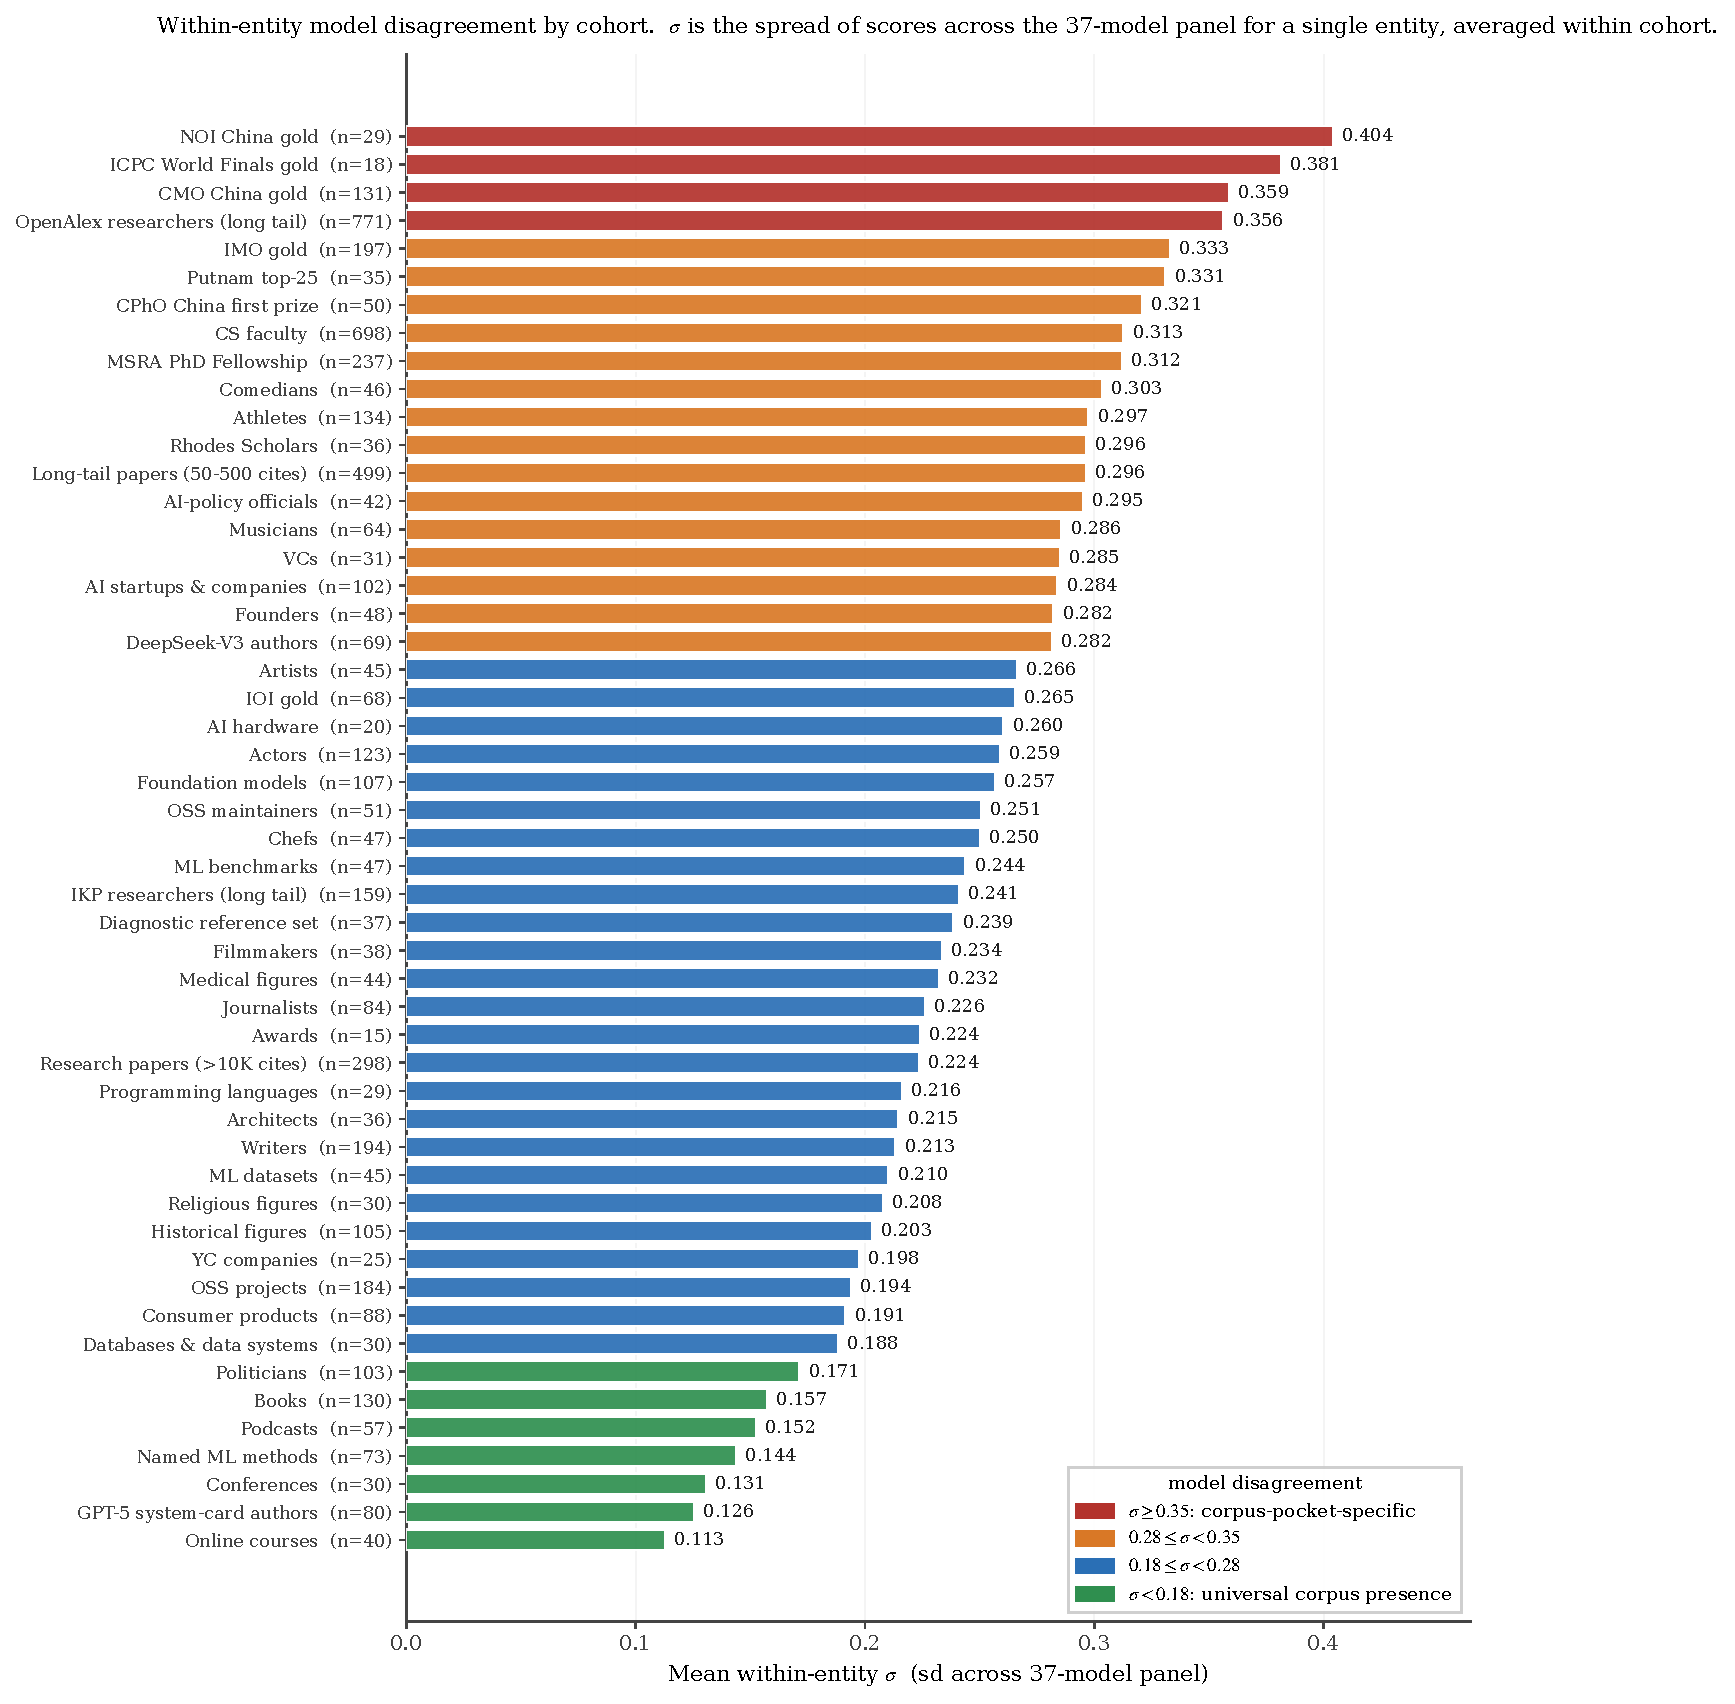
\includegraphics[width=0.92\textwidth]{figures/fig_app_sigma.pdf}
    \caption{Full within-entity $\sigma$ ladder across all cohorts with $n \geq 10$. Color bands group cohorts by the four $\sigma$ regimes (universal $\to$ corpus-pocket-specific). The high-$\sigma$ end is dominated by competition-credential and long-tail academic cohorts whose recognition is genuinely corpus-fragment-specific; the low-$\sigma$ end is dominated by entities whose names appear in nearly every training source (online courses, conferences, named methods, books).}
    \label{fig:app-sigma}
\end{figure}

The variance pattern is itself a probe of corpus-pocket distribution: cohorts with high $\sigma$ are the ones where ``which model do you ask?'' changes the answer.

% ══════════════════════════════════════════════════════════════
\section{Prompt-Paraphrase Sensitivity}
\label{app:prompt-sensitivity}

We re-probed a cohort-stratified $200$-entity subset ($30$ each from IMO gold, OpenAlex long-tail researchers, CS faculty, Writers, OSS projects, GPT-5 system-card authors; $10$ each from Research papers and Filmmakers) on the full $37$-model panel under three paraphrased probe templates (T1--T3) alongside the original (T0), for $29{,}600$ records. The four templates:

\begin{verbatim}
T0: Tell me what you know about {name}, who is {context}. If you do
    not recognize this entity, respond with "unknown". Limit your
    response to about 150 words.
T1: What can you tell me about {name}? They are {context}. Reply with
    only "unknown" if you are not familiar with this entity. Aim for
    about 150 words.
T2: Please share what you know about {name}, {context}. If unknown to
    you, answer with just "unknown". Keep it under ~150 words.
T3: Briefly describe {name}, who is {context}. Respond "unknown" if
    you have no information. Around 150 words please.
\end{verbatim}

\begin{table}[!htbp]
\centering
\small
\caption{Additive variance decomposition over the $29{,}600$ prompt-sensitivity records (entity, model, template, cohort as main effects). Template is the smallest main effect. The model share exceeds the full-panel $10.9\%$ (Section~\ref{sec:results-validation}) because this cohort-stratified subset over-represents silent and universal cohorts, compressing the entity-vs-model contrast; the valid within-experiment comparison is template ($1.78\%$) vs model ($26.5\%$).}
\label{tab:prompt-variance}
\begin{tabular}{lrr}
\toprule
Factor & SS & \% of total \\
\midrule
Entity & 985.3 & 24.19\% \\
Model & 1079.9 & 26.51\% \\
Cohort (entity-implied) & 551.9 & 13.55\% \\
\textbf{Template} & \textbf{72.4} & \textbf{1.78\%} \\
Residual (after entity+model+template) & 1936.3 & 47.53\% \\
\bottomrule
\end{tabular}
\end{table}

\begin{table}[!htbp]
\centering
\small
\caption{Cohort-mean NameRank under each template (sorted by T0). The ordering is preserved; T0 is systematically higher. Pairwise panel-mean Pearson across all six template pairs is $0.927$--$0.977$ (lowest: T0--T3); within-(entity, model) cross-template $\sigma$ has median $0.109$; the panel-mean variance across templates is $0.042\times$ the single-template cross-model variance.}
\label{tab:prompt-cohort-means}
\begin{tabular}{lrrrr}
\toprule
Cohort & T0 & T1 & T2 & T3 \\
\midrule
Filmmakers & 0.761 & 0.506 & 0.513 & 0.532 \\
Writers & 0.597 & 0.388 & 0.403 & 0.405 \\
Research papers & 0.581 & 0.391 & 0.394 & 0.401 \\
OSS projects & 0.504 & 0.334 & 0.335 & 0.331 \\
OpenAlex long-tail researchers & 0.465 & 0.362 & 0.341 & 0.455 \\
CS faculty & 0.384 & 0.300 & 0.295 & 0.319 \\
IMO gold & 0.356 & 0.290 & 0.260 & 0.302 \\
GPT-5 system-card authors & 0.047 & 0.063 & 0.027 & 0.070 \\
\midrule
\textbf{Panel template mean} & \textbf{0.420} & \textbf{0.305} & \textbf{0.294} & \textbf{0.329} \\
\bottomrule
\end{tabular}
\end{table}

\section{Training-Cutoff Gradient}
\label{app:cutoff}

The two first-appearance cohorts (DeepSeek-V3 authors, emergence 2024-12; GPT-5 system-card authors, emergence 2025-08) test whether the silent zone is corpus timing or intrinsic obscurity (Section~\ref{sec:results-cutoff}). Model training cutoffs are from \texttt{data/analysis/model\_cutoffs.json} and span 2023-10 to 2026-03.

\begin{table}[!htbp]
\centering
\small
\caption{Natural experiment: per-model mean recognition split by whether the model's training cutoff predates (pre) or postdates (post) each cohort's emergence date. The raw jump is decomposed by a matched difference-in-differences (DiD) that subtracts the same-split jump averaged over three stable controls (CS faculty, OpenAlex long-tail researchers, IMO gold), which nets out the cross-vintage capability drift. Both matched DiDs are $\leq 0$.}
\label{tab:cutoff-natexp}
\begin{tabular}{lrrrrr}
\toprule
Cohort & pre (refusal) & post (refusal) & raw jump & control & DiD \\
\midrule
DeepSeek-V3 authors & 0.113 (0.38) & 0.233 (0.45) & $+0.121$ & $+0.137$ & $\mathbf{-0.016}$ \\
GPT-5 system-card authors & 0.051 (0.49) & 0.020 (0.79) & $-0.031$ & $+0.030$ & $\mathbf{-0.061}$ \\
\bottomrule
\end{tabular}
\end{table}

\begin{table}[!htbp]
\centering
\small
\caption{Selected per-cohort slopes of per-model mean NameRank on training cutoff (NameRank per year of cutoff), with Pearson $r$ over the $37$ models. \emph{Every} established cohort rises with cutoff at ${\sim}0.10$--$0.20$/yr---a model-capability/generosity confound, since these entities were nameable long before any cutoff. The two recency cohorts are \emph{not} steeper; once the drift is removed (Table~\ref{tab:cutoff-natexp}) no corpus-timing signal remains.}
\label{tab:cutoff-slopes}
\begin{tabular}{lrr}
\toprule
Cohort & slope (/yr) & Pearson $r$ \\
\midrule
Comedians & $+0.196$ & $+0.66$ \\
Foundation models & $+0.171$ & $+0.76$ \\
CS faculty (control) & $+0.158$ & $+0.57$ \\
Reference set (control; incl.\ Hinton) & $+0.157$ & $+0.77$ \\
Research papers & $+0.125$ & $+0.74$ \\
OpenAlex long-tail researchers (control) & $+0.094$ & $+0.32$ \\
\textbf{DeepSeek-V3 authors} (recency) & $+0.065$ & $+0.23$ \\
IMO gold & $+0.043$ & $+0.15$ \\
\textbf{GPT-5 system-card authors} (recency) & $-0.021$ & $-0.25$ \\
\bottomrule
\end{tabular}
\end{table}

\section{Bibliometric Predictor Decomposition}
\label{app:bibliometric}

Six bibliometric predictors regressed on NameRank for the $n = 771$ OpenAlex long-tail cohort (Section~\ref{sec:results-external}), testing whether $h$-index dominates because it discounts per-paper name attribution. \texttt{fractional\_citations} divides each paper's citations by its author count; \texttt{first\_last\_citations} counts only papers where the researcher is first or last author; \texttt{n\_works} is the raw count of works; \texttt{mean\_authors} is the mean author count per paper. All $R^2$ on $\log(1+x)$-transformed predictors.

\begin{table}[!htbp]
\centering
\small
\caption{Sole-predictor $R^2$ on NameRank and marginal $R^2$ when added to $h$-index alone. Attribution-weighted measures (fractional, first/last) do not approach $h$-index, and add almost nothing on top of it; author count carries no signal. The count of distinct works ($n_\text{works}$) is the closest cousin of $h$-index.}
\label{tab:bibliometric}
\begin{tabular}{lrr}
\toprule
Predictor & Sole $R^2$ & $\Delta R^2$ added to $h$-index \\
\midrule
$\log(h\text{-index})$ & \textbf{0.398} & --- \\
$\log(n_\text{works})$ & 0.337 & $+0.0003$ \\
$\log(\text{first/last-author citations})$ & 0.268 & $+0.0268$ \\
$\log(\text{fractional citations})$ & 0.154 & $+0.0026$ \\
$\log(\text{raw citations})$ & 0.137 & $+0.0001$ \\
$\log(\text{mean authors/paper})$ & 0.0004 & $+0.0008$ \\
\bottomrule
\end{tabular}
\end{table}

In a joint OLS over all six (total $R^2 = 0.428$), the standardized coefficients are dominated by $\log(h\text{-index})$ ($0.579$), with first/last-author citations ($0.202$) a distant second and raw citations \emph{negative} ($-0.143$); fractional citations ($0.109$) and mean authors ($0.060$) are minor. The mechanism is name-recurrence across distinct works, not attribution-per-paper weighting: if the latter drove the result, fractional and first/last-author citations would match or exceed $h$-index, and they do not.

\section{Cross-Judge Robustness}
\label{app:cross-judge}

A $615$-record stratified sample (Section~\ref{sec:results-judge}) was re-graded by Claude Opus 4.6 and GPT-5.5 alongside the primary Gemini 3 Flash Preview judge, holding gold answers and judge prompt fixed.

\begin{table}[!htbp]
\centering
\small
\caption{Pairwise Pearson correlation between judges, by cohort. Agreement is high everywhere except the $n = 15$ OSS projects cell (generic-description disagreement). The Reference set anchors---including its four Chinese-name entities---show the tightest agreement, refuting a ``Chinese name $\to$ judge disagreement'' hypothesis.}
\label{tab:cross-judge-corr}
\begin{tabular}{lrrrr}
\toprule
Subset & $n$ & Gem--Claude & Gem--GPT-5 & Claude--GPT-5 \\
\midrule
ALL & 615 & 0.868 & 0.893 & 0.934 \\
Reference set & 185 & 0.952 & 0.941 & 0.972 \\
\quad (Chinese-name subset) & 74 & 0.957 & 0.945 & 0.970 \\
OpenAlex long-tail researchers & 100 & 0.855 & 0.920 & 0.935 \\
CS faculty & 100 & 0.712 & 0.894 & 0.781 \\
IMO gold & 100 & 0.785 & 0.808 & 0.924 \\
GPT-5 system-card authors & 100 & 0.781 & 0.917 & 0.830 \\
Writers & 15 & 0.872 & 0.853 & 0.878 \\
OSS projects & 15 & 0.103 & 0.455 & 0.486 \\
\bottomrule
\end{tabular}
\end{table}

\begin{table}[!htbp]
\centering
\small
\caption{Capability-controlled in-family lift. For each response, a judge's score is compared to the mean of the \emph{other two} judges on that same response; the lift is the own-family residual minus the other-family residual. Gemini and GPT-5 modestly favor their own family; Claude does not.}
\label{tab:cross-judge-bias}
\begin{tabular}{lrrr}
\toprule
Judge & In-family residual & Other-family residual & Lift \\
\midrule
Gemini & $+0.014$ & $-0.048$ & $\mathbf{+0.062}$ \\
GPT-5 & $+0.060$ & $+0.019$ & $\mathbf{+0.041}$ \\
Claude & $+0.012$ & $+0.022$ & $\mathbf{-0.010}$ \\
\bottomrule
\end{tabular}
\end{table}

Cohort-mean NameRank is stable across judges, and the silent$\to$discriminative$\to$universal ladder is preserved under all three: on this stratified $615$-record subsample (whose per-cohort means differ from the full-run means by construction), the GPT-5 system-card cohort scores $0.087$/$0.165$/$0.123$ under Gemini/Claude/GPT-5, and the OpenAlex long-tail cohort $0.669$/$0.630$/$0.631$. The headline findings are not a single-judge artifact.

\section{Synthetic-Null Floor}
\label{app:synthetic}

Thirty fictional entities (ungoogleable names verified to surface no notable real person; cohort-matched contexts and gold answers) were run through the full pipeline (Section~\ref{sec:results-synthetic}). Table~\ref{tab:synthetic} gives the per-archetype floor.

\begin{table}[!htbp]
\centering
\small
\caption{Synthetic-null mean NameRank by archetype. Dense-gold archetypes (founder, CS faculty) floor near the main-run silent level; the short-boilerplate-gold IMO archetype floors much higher, because its generic year$+$country$+$medal gold is partly satisfiable from the disambiguating context without recognizing the (nonexistent) person.}
\label{tab:synthetic}
\begin{tabular}{lrrr}
\toprule
Synthetic archetype & $n$ & Mean NameRank & Refusal \\
\midrule
IMO gold (boilerplate gold) & 6 & \textbf{0.199} & 21\% \\
Chef & 1 & 0.123 & 27\% \\
Journalist & 1 & 0.092 & 27\% \\
Podcast & 1 & 0.075 & 32\% \\
OSS project & 4 & 0.065 & 39\% \\
Musician & 1 & 0.057 & 41\% \\
CS faculty & 10 & \textbf{0.027} & 45\% \\
Founders & 6 & \textbf{0.012} & 47\% \\
\midrule
All synthetics & 30 & 0.072 & --- \\
All except IMO archetype & 24 & \textbf{0.040} & --- \\
\bottomrule
\end{tabular}
\end{table}

The floor is concentrated in small open-weights fluent hallucinators: gemma-3-4b ($0.293$), gemma-3-12b ($0.287$), and llama-4-maverick ($0.259$) lead, while $15$ of the $37$ models score the synthetics at exactly $0$ (including grok-4, kimi-k2, qwen3-235b, mistral-large, gemini-3.1-pro, and gpt-5.3, the last two by refusing on $100\%$ of synthetics). Recommended use: treat $\sim 0.04$ as the noise floor for dense-gold cohorts and $\sim 0.20$ for short-boilerplate-gold cohorts; differences below the relevant floor are not evidence of recognition.

\section{Confound Checks: Gold Length, Context, and Wikipedia}
\label{app:confounds}

\textbf{Gold-answer length.} Within-cohort regressions of NameRank on gold-answer length give $R^2 < 0.07$ for IMO ($0.067$), IOI ($0.018$), and MSRA ($0.006$); the high-$R^2$ cohorts are fame-graded mid-tier categories (actor $0.95$, writer $0.88$) where longer golds are an outcome of fame, not a measurement artifact. The credential-vs-OpenAlex ordering survives a pooled fixed-effects length adjustment (which deepens the gap: pooled slope $b_\text{chars} = -1.1{\times}10^{-3}$) and a within-OpenAlex-slope adjustment. A strict $|\Delta\text{chars}| \leq 50$ matched-pairs test yields $n = 0$ pairs: IMO golds span $359$--$392$ characters, OpenAlex golds $662$--$789$, with no overlap. The closest feasible match (IMO vs.\ CMO, which do overlap in length) preserves the within-credential ordering.

\textbf{Disambiguating context.} A $288$-entity subset re-probed with the specific context replaced by a minimal generic descriptor:

\begin{table}[!htbp]
\centering
\small
\caption{Minimal-context ablation. Stripping the specific disambiguating context to a generic descriptor drops absolute NameRank substantially but preserves the cross-entity gradient.}
\label{tab:context}
\begin{tabular}{lrr}
\toprule
Comparison & Specific context & Minimal context \\
\midrule
OpenAlex long-tail researchers (mean) & 0.446 & 0.077 \\
IMO gold (mean) & 0.345 & 0.039 \\
Stanford mean & 0.565 & 0.355 \\
Tsinghua mean & 0.258 & 0.062 \\
\textbf{Stanford$-$Tsinghua gap} & \textbf{0.308} & \textbf{0.293} ($-4.8\%$) \\
\bottomrule
\end{tabular}
\end{table}

Absolute levels fall sharply (the model cannot identify which researcher without the context), but the Stanford--Tsinghua institutional gap shrinks by only $\sim 5\%$: context anchors disambiguation, it does not leak the gold answer.

\textbf{Wikipedia presence.} On the $n = 771$ long-tail cohort, a binary has-Wikipedia flag explains $R^2 = 0.022$ of NameRank (log-sitelinks and log-pageviews add $+0.007$ and $0.000$ on top), versus $R^2 = 0.398$ for $\log(h\text{-index})$ alone. Adding $\log(h\text{-index})$ to the full Wikipedia block lifts $R^2$ from $0.029$ to $0.405$---a marginal $R^2$ of $0.376$. Across the full $5{,}719$-entity cohort, Wikipedia presence explains $\sim 8\%$ of variance and cohort identity $\sim 47\%$. Wikipedia presence accounts for only $\sim 1/4$ of the Stanford--Tsinghua gap. NameRank tracks bibliometric productivity, not a Wikipedia-yes/no flag.

\section{Gender Gap by Cohort}
\label{app:gender}

First-name-inferred gender (via \texttt{gender-guesser}; ambiguous and unisex names dropped) for the person cohorts, restricted to cohorts with $\geq 5$ man- and woman-coded names. Table~\ref{tab:gender} reports the man-minus-woman NameRank gap.

\begin{table}[!htbp]
\centering
\small
\caption{Man-minus-woman NameRank gap by cohort. The controlled researcher cohorts (top) show a small reproducible man-coded advantage that survives institution- and $h$-index-matching. The cross-profession cohorts (bottom) show much larger raw gaps that reflect real-world fame differences in the sampled individuals, not a NameRank artifact---hence the bias claim is restricted to the controlled researcher comparison.}
\label{tab:gender}
\begin{tabular}{lrrrr}
\toprule
Cohort & $n_\text{man}$ & $n_\text{woman}$ & $\Delta$ (man$-$woman) & $p$ \\
\midrule
CS faculty & 354 & 97 & $+0.038$ & 0.014 \\
\quad institution-matched ($60$ pairs) & --- & --- & $+0.054$ & 0.042 \\
OpenAlex long-tail researchers & 388 & 76 & $+0.031$ & 0.182 \\
\quad $h$-index-decile-adjusted & --- & --- & $+0.032$ & --- \\
IKP long-tail researchers & 56 & 22 & $+0.044$ & 0.015 \\
\midrule
Actors & 38 & 63 & $+0.341$ & $<10^{-3}$ \\
Athletes & 64 & 32 & $+0.254$ & $<10^{-3}$ \\
Writers & 62 & 77 & $+0.041$ & 0.41 \\
Comedians & 18 & 17 & $-0.045$ & 0.23 \\
\bottomrule
\end{tabular}
\end{table}

The within-researcher-cohort gap ($+0.027$ to $+0.054$, ${\sim}6$--$8\%$ relative attenuation) is roughly $4\times$ smaller than the ${\sim}2\times$ East-Asian-surname attenuation reported by \citet{li2026ikp}, but reproducible across three researcher cohorts and robust to dropping medium-confidence gender labels. The large cross-profession gaps (actor, athlete) are excluded from the bias claim because the sampled men and women in those cohorts differ in actual fame.

\textbf{Name-coding caveat.} \texttt{gender-guesser} infers gender from first names against a predominantly Western-name dictionary; it returns ``unknown'' or ``andy'' (androgynous) for most Chinese, Korean, and other romanized East-Asian given names, which are then dropped. The gendered sub-sample is therefore enriched for Western names, and the residual gender gap is partly entangled with the East-Asian-surname attenuation it sits beside---a name that codes as gender-unknown also tends to be one of the low-recognition non-Anglophone names. The $n_\text{woman}$ counts (e.g.\ $76$--$97$ across the researcher cohorts) reflect this attrition. We report the gap as an inherited corpus-and-judge property restricted to the controlled within-cohort comparison, not as a clean estimate of a pure gender effect net of name origin; disentangling the two would require a gender labeling that is accurate on CJK names (e.g.\ manual coding or a name-origin-aware classifier).

\section{News-Event Cohort: Construction and Detail}
\label{app:events}

This appendix documents the construction of the $258$-event cohort of Section~\ref{sec:results-events} and reports the full tables behind its findings. All construction scripts, inputs, and derived data are released under \texttt{experiments/t4\_1\_news\_events/} in the repository.

\subsection{Sampling frame and filters}

Candidate events are harvested from the ``Events'' sections of the English Wikipedia year articles (\emph{2021}, \emph{2022}, \emph{2023}) and of $32$ country-year articles (``\emph{2021 in India}'', ``\emph{2022 in Nigeria}'', \ldots) chosen to balance nine world regions ($2{,}245$ unique linked articles). Each candidate is classified by Gemini~3 Flash Preview (the study's judge family; temperature $0$, structured output) from its title, short description, and first paragraph into: discrete event or not, start year and month, primary country, region, and category. An article qualifies as a \emph{discrete event} if it describes a specific occurrence or tightly bounded series (an election, a storm, a trial, a tournament, an accident, a protest wave) that began at an identifiable date; people, organizations, products, laws, ongoing multi-year topics, and list/timeline articles are excluded ($1{,}041$ qualify). Post-classification filters require a standard-type article with an intro of $\geq 40$ words and a first-year pageview record of $\geq 1{,}000$ total views over $\geq 200$ recorded days; $655$ events survive. Stratifying by $\log_{10}$(total views) band ($<10^4$ through $\geq 10^7$) crossed with eight region groups, capped at $14$ events per cell, yields the released cohort of $258$.

\subsection{Attention measures and cross-checks}

For each event we retrieve the daily en-Wikipedia pageview series of its article (Wikimedia REST API, user traffic only) for the $365$ days from the first day of the event's start month, and define \textbf{total attention} (summed daily views), \textbf{peak attention} (maximum daily views), and \textbf{effective duration} $=$ total$/$peak in days, linked by the identity $\log(\text{total}) = \log(\text{peak}) + \log(\text{duration})$. Wikipedia pageviews are a standard collective-attention proxy~\citep{mestyan2013early,ripberger2011capturing}; we prefer them to Google Trends because the pageview record is absolute, archived, and reproducible, whereas the public Trends interface returns only normalized indices under heavy rate limits. Two caveats. First, the ledger is attention \emph{to the event's English Wikipedia article}, so all matched-attention comparisons condition on English-audience interest; this is a feature for the region analysis (it holds English exposure fixed) but means globally quiet, locally enormous events enter as quiet. Second, attention can fragment across sibling articles (\emph{Killing of Tyre Nichols} vs.\ \emph{Tyre Nichols protests}), adding measurement noise that biases dose--response estimates toward zero. A GDELT news-coverage-volume cross-check~\citep{leetaru2013gdelt} on the event's name phrase over the same window is reported under Full Results below and released with the data (\texttt{outputs/gdelt.json}).

\subsection{Probes and panel}

Golds are the article's intro truncated to $100$--$200$ words at a sentence boundary (the main run's Wikipedia gold recipe); disambiguating contexts are generated deterministically from the classification fields only---category phrase, location, month, year---never from article content, mirroring the main run's role/affiliation/field rule. Probe template, judge model, judge prompt, refusal detection, and scoring are unchanged from Section~\ref{sec:method}.

\textbf{Panel.} Nine of the $37$ main-run models could not complete the event run ($2026$-$07$): eight lost all OpenRouter routing to provider delistings and deprecations (Ernie-4.5-300b, Mistral-Large-2411, Mistral-Medium-3.1, Ministral-3b, Kimi-K2, Grok-4, GLM-4-32b, Llama-3.2-1b), and Grok-4.20-think---initially recovered via the direct xAI API---lost access when that account exhausted its credits at $143$ of $258$ events, so its partial coverage is discarded (a model must cover the full cohort to enter the panel mean). The eight delisted models are replaced by the representative newly released models evaluated in the IKP revision~\citep{li2026ikp}: Claude Fable 5, GLM-5.2, Qwen3.7-Max, Kimi-K2.7-code, MiniMax-M3, Step-3.7-Flash, Nemotron-3-Ultra-550b, and Nemotron-3-Nano-30b (one representative per newly covered vendor family, plus a second NVIDIA entry to restore the small-model tier lost with Ministral-3b and Llama-3.2-1b; all run in thinking mode per the panel policy). Event NameRank is therefore a $36$-model panel mean ($28$ survivors $+$ $8$ replacements) over $9{,}288$ records. Neither change matters for comparability. Recomputing the full main run on the $28$-model surviving sub-panel correlates with the released $37$-model scores at $r = 0.993$ per entity (mean shift $+0.011$), so main-run numbers are quoted unadjusted alongside event scores, and cross-run placements use survivor-only event means. And the replacements reproduce the survivors' ordering: per-event means over the $8$ new models correlate at $r = 0.905$ with means over the $28$ survivors (level shift $+0.091$---the $2026$-vintage models are uniformly more knowledgeable about $2021$--$2023$ events), the entity-not-panel property of Section~\ref{sec:val-variance} on models released a year apart.

\textbf{Cutoff coverage.} Three panel models have training cutoffs inside the final months of the event window (Mistral-Small-24b, $2023$-$10$; Llama-3.1-8b and Llama-3.3-70b, $2023$-$12$); the eight replacement models are $2026$ releases with cutoffs far past the window. Neither exclusion matters: dropping the $22$ events that begin in October--December $2023$ leaves the joint attention decomposition at peak $+0.045$ / duration $-0.007$; dropping the three models for all events gives $+0.038$ / $-0.009$ (vs.\ $+0.042$ / $-0.008$ headline).

\subsection{Full results}

\textbf{Dose--response.} Table~\ref{tab:events-deciles} gives the decile ladder with the coverage/accuracy channel decomposition. Sole-predictor $R^2$ on NameRank: $\log$ total views $0.095$ (repeated $10$-fold CV $0.09 \pm 0.11$), $\log$ peak $0.119$ ($0.11 \pm 0.12$), $\log$ effective duration $0.033$ ($0.02 \pm 0.08$), $\log$ tail interest (mean daily views in days $300$--$365$) $0.065$. Gold length alone explains $0.006$; adding it to $\log$ total views raises $R^2$ to $0.168$ and the attention slope from $+0.042$ to $+0.063$ per decade (gold density suppresses).

\begin{table}[!htbp]
\centering
\small
\caption{NameRank by decile of total first-year pageviews ($n = 258$). Attention converts refusal into accurate specifics: accuracy rises steeply, coverage gently.}
\label{tab:events-deciles}
\begin{tabular}{rrrrrr}
\toprule
Decile & $n$ & Geo.\ mean views & NameRank & Refusal & (cov, acc) \\
\midrule
D1 & 25 & 2{,}415 & 0.379 & 0.12 & (0.46, 0.61) \\
D2 & 26 & 7{,}395 & 0.385 & 0.11 & (0.47, 0.60) \\
D3 & 26 & 16{,}514 & 0.405 & 0.12 & (0.46, 0.64) \\
D4 & 26 & 39{,}348 & 0.464 & 0.07 & (0.54, 0.67) \\
D5 & 26 & 67{,}583 & 0.427 & 0.06 & (0.49, 0.71) \\
D6 & 25 & 133{,}127 & 0.513 & 0.05 & (0.57, 0.75) \\
D7 & 26 & 251{,}374 & 0.484 & 0.04 & (0.55, 0.78) \\
D8 & 26 & 480{,}323 & 0.478 & 0.01 & (0.53, 0.85) \\
D9 & 26 & 1{,}223{,}071 & 0.490 & 0.01 & (0.54, 0.85) \\
D10 & 26 & 3{,}312{,}033 & 0.499 & 0.01 & (0.54, 0.88) \\
\bottomrule
\end{tabular}
\end{table}

\textbf{Peak vs.\ duration.} Joint regression of NameRank on the standardized log-components: peak $+0.042$ (HC1 se $0.008$), duration $-0.008$ (se $0.009$), joint $R^2 = 0.122$ (CV $0.11 \pm 0.12$); marginal $R^2$ of duration given peak $= 0.003$. With recurring-name and gold-length controls: peak $+0.070$ (se $0.012$), duration $+0.005$ (se $0.010$). Within peak terciles, moving from the shortest to the longest duration tercile moves NameRank by $-0.07$, $+0.01$, and $-0.01$ respectively---no duration channel at matched peak.

\textbf{Recurring-series flag.} An event is a series instance if substituting a nearby year (or adjacent ordinal/Roman edition marker) into its title yields another standard Wikipedia article; the detector sweeps $y \pm 1..6$ to cover $4$--$6$-year election cycles. $106$ of $258$ events flag as recurring; at matched attention the penalty is $-0.061$ (se $0.015$). The flag is conservative---renamed series (\emph{2023 Men's FIH Hockey World Cup} vs.\ \emph{2018 Men's Hockey World Cup}) escape detection and dilute the estimate.

\textbf{Region and vintage.} Table~\ref{tab:events-region} reports raw and attention-adjusted region contrasts. Event-year effects at matched attention: $2022$ vs.\ $2021$: $-0.009$ (se $0.019$); $2023$ vs.\ $2021$: $-0.049$ (se $0.018$).

\textbf{GDELT cross-check.} Of the $258$ name-phrase queries, the rate-limited GDELT DOC API returned data for $159$; $118$ had nonzero matched coverage. On those, $\log$ GDELT coverage volume correlates with $\log$ pageviews at $r = 0.33$---the two ledgers partially agree---but predicts NameRank at only $R^2 = 0.006$. We attribute the gap mostly to query noise: GDELT matches the event's literal name phrase, which misses paraphrase references and truncates awkwardly for long titles, and the returned subset is rate-limit-selected rather than random. We therefore rely on the pageview ledger and report GDELT as a weak consistency check on the attention record, not an independent predictor.

\begin{table}[!htbp]
\centering
\small
\caption{Region groups: raw mean NameRank and the adjusted delta vs.\ the Anglo-America \& Oceania baseline after controlling $\log_{10}$ total views (HC1 standard errors). The single Global-classified event (the Queen's Platinum Jubilee Beacons) is omitted.}
\label{tab:events-region}
\begin{tabular}{lrrr}
\toprule
Region group & $n$ & Raw mean & Adj.\ $\Delta$ (se) \\
\midrule
Anglo-America \& Oceania & 45 & 0.463 & (baseline) \\
Eastern Europe \& Russia & 28 & 0.506 & $+0.038$ (0.030) \\
Middle East \& Africa & 35 & 0.480 & $+0.009$ (0.028) \\
Western Europe & 44 & 0.453 & $-0.013$ (0.025) \\
Latin America & 32 & 0.452 & $-0.008$ (0.026) \\
East Asia & 31 & 0.425 & $-0.033$ (0.031) \\
South \& Southeast Asia & 42 & 0.397 & $-0.060$ (0.028) \\
\bottomrule
\end{tabular}
\end{table}

% ══════════════════════════════════════════════════════════════
\section{Limitations Summary Table}
\label{app:limitations}

\begin{table}[!htbp]
\centering
\footnotesize
\caption{Compact summary of methodological caveats, their direction (could overstate or understate findings), and mitigations available for future runs.}
\label{tab:limitations}
\begin{tabular}{>{\raggedright\arraybackslash}p{4.3cm}>{\raggedright\arraybackslash}p{4.3cm}>{\raggedright\arraybackslash}p{5.9cm}}
\toprule
\textbf{Caveat} & \textbf{Direction} & \textbf{Mitigation} \\
\midrule
Single-probe-per-entity; absolute levels are wording-conditional (Appendix~\ref{app:prompt-sensitivity}) & Shifts cardinal levels ${\sim}0.10$--$0.20$; rankings unaffected & \emph{Tested:} four-template re-probe shows ordering robust ($r = 0.93$--$0.98$); report values as T0-conditional and hold wording fixed across studies \\
Judge family-bias (Appendix~\ref{app:cross-judge}) & Gemini-judging-Gemini lift $+0.062$ inflates per-vendor score tables; cross-entity findings unaffected & \emph{Tested:} 3-judge re-grade ($n=615$); report per-vendor tables under Claude or as a 3-judge mean \\
Cohort labels not fully orthogonal & Overcounts entities in cross-cohort comparisons & De-duplicate by name within long-tail academic categories \\
Chinese-prompt context fields remained English & Understates cross-language effect & Pure-Chinese prompts for the full $240$-entity sub-run \\
Single judge on the full run (Gemini 3 Flash Preview) & Family-specific scoring style on per-vendor tables & \emph{Tested:} non-Gemini replication (Claude, GPT-5) on $n = 615$; a full multi-judge consensus run would remove the offset \\
Cross-section, not longitudinal & Cannot infer name-propagation rates & Re-run at each major model-release cycle; release as NameRank v2, v3, ... \\
Scores not comparable across model vintages (Appendix~\ref{app:cutoff}) & ${\sim}0.13$/yr capability drift inflates any cross-fleet level comparison & \emph{Tested:} silent zone is intrinsic, not timing (matched DiD ${\approx}0$); make longitudinal claims on within-run relative gaps only \\
Researcher mobility confound in country gradient & Inflates US averages, deflates China averages & Re-classify by country-of-PhD or country-of-doctorate-training as alternative slicing \\
Tsinghua/Peking small samples ($n = 4$) & Institution-level reads noisy at the bottom & Expand sample by drawing from CCF rank-A faculty rosters \\
Tianshou case study sample of $1$ for per-response mediation analysis & Cannot generalize the $+0.36$ score lift cleanly & Extend per-response mediation analysis to all $11$ verified (creator, artifact) pairs \\
Inherited gender bias (Appendix~\ref{app:gender}) & Man-coded researcher names score $+0.03$--$0.05$ over woman-coded & \emph{Measured, not corrected:} report alongside the East-Asian-surname effect; restrict to controlled within-cohort comparisons \\
Short-boilerplate-gold cohorts have an elevated noise floor (Appendix~\ref{app:synthetic}) & Olympiad-credential scores up to $\sim 0.20$ are partly context-prior leakage & Read scores against the synthetic floor ($\sim 0.04$ dense-gold, $\sim 0.20$ short-gold); the floor widens, not narrows, the credential gap \\
Institution variance share inflated by category count (Section~\ref{sec:results-geography}) & Naive $R^2 = 0.54$ counts $319$ dummies on $698$ points; true share ${\sim}16\%$ & \emph{Corrected:} report adjusted $R^2$/$\omega^2$/ICC (${\sim}0.16$) and the large-cell Stanford--Tsinghua contrast; country-level aggregation is not inflated \\
Context-injection lift includes a coverage-echo component (Section~\ref{sec:results-mediation-causal}) & Overstates the named-artifact-amplification effect; lift is an upper bound & Re-judge arm~B against an artifact-redacted gold crediting only non-injected facts; report the residual lift \\
Gold/training-source overlap for Wikipedia-derived golds (Section~\ref{sec:method}) & For ${\sim}60\%$ of entities, coverage partly measures Wikipedia memorization & \emph{Tested:} a binary Wikipedia flag explains only ${\sim}2\%$ of long-tail variance vs.\ $40\%$ for $h$-index (Appendix~\ref{app:confounds}) \\
Event attention ledger conditions on English-Wikipedia interest (Appendix~\ref{app:events}) & Matched-attention region contrasts hold English exposure fixed; globally quiet, locally enormous events enter as quiet & Add non-English pageview ledgers (major Wikipedia editions) as parallel exposure measures \\
Event attention fragments across sibling articles (Appendix~\ref{app:events}) & Attenuates the dose--response slope toward zero & Aggregate pageviews over each event's article cluster before computing the ledger \\
Event panel differs from the main-run panel ($36$ models: $28$ survivors $+$ $8$ replacements) & Cross-run level comparisons shift ($+0.011$ survivors, $+0.091$ replacements) & \emph{Tested:} survivor sub-panel $r = 0.993$ with released scores; replacements rank events at $r = 0.905$; quote cross-run placements on the survivor sub-panel \\
\bottomrule
\end{tabular}
\end{table}


\end{document}
